\documentclass[11pt,a4paper]{article}
\usepackage{graphicx}
\usepackage{ctex}
\usepackage{indentfirst}
%\graphicspath{{chapter/}{figures/}}
\usepackage{CJK}
\usepackage{amsmath}%数学
\usepackage{cite}%参考文献
\usepackage{graphicx} %插入图片的宏包
\usepackage{float} %设置图片浮动位置的宏包
\usepackage{subfigure} %插入多图时用子图显示的宏包
\graphicspath{ {figure/} }

\usepackage{appendix}%附录
% \usepackage{tabularx}%表格

\usepackage{pdfpages}%插入pdf

\usepackage{dirtree}%文件目录树

\usepackage{makecell}%表格竖线连续
\newcommand\toprule{\Xhline{.08em}}
\newcommand\midrule{\Xhline{.05em}}
\newcommand\bottomrule{\Xhline{.08em}}
\def\I{\vrule width1.2pt}
%!\I 就可以代替| 来画表格了

%可固定下划线长度
\makeatletter
\newcommand\dlmu[2][4cm]{\hskip1pt\underline{\hb@xt@ #1{\hss#2\hss}}\hskip3pt}
\makeatother


\usepackage{array}%数学
\usepackage{multirow}%跨行表格
%\usepackage[colorlinks,linkcolor=red]{hyperref}%超链接

\usepackage{fancyhdr}  %使用fancyhdr包自定义页眉页脚
%\pagestyle{empty}
\pagestyle{fancy}
%\pagestyle{plain}%没有页眉,页脚放页数
\renewcommand{\headrulewidth}{0.5pt}
\renewcommand{\footrulewidth}{0.4pt}
\lhead{}
\chead{}
\rhead{}
\lfoot{}
\cfoot{\thepage}
\rfoot{}


\usepackage{booktabs}%表格用

\usepackage{float}%可以用于禁止浮动体浮动

%目录超链接
\usepackage[colorlinks,linkcolor=black,anchorcolor=blue,citecolor=black]{hyperref}

\usepackage{listings}%可以插入代码
\usepackage{xcolor}%语法高亮支持
%代码格式
\definecolor{dkgreen}{rgb}{0,0.6,0}
\definecolor{gray}{rgb}{0.5,0.5,0.5}
\definecolor{mauve}{rgb}{0.58,0,0.82}
\lstset{ %
	%	language=Python,                % the language of the code
	breaklines,%自动折行
	%extendedchars=false%解决代码跨页时,章节标题,页眉等汉字不显示的问题
	keepspaces=false,  
	%tabsize=4 %设置tab空格数
	showspaces=false,  %不显示空格
	showtabs=false,  
	showstringspaces=true, 
	numbers=left, 
	basicstyle=\footnotesize, 
	numberstyle=\tiny, 
	numbersep=5pt, 
	keywordstyle= \color{ blue!70},%关键字颜色
	commentstyle= \color{red!50!green!50!blue!50},%注释颜色 
	frame=shadowbox, % 边框格式:阴影效果
	rulesepcolor= \color{ red!20!green!20!blue!20} ,
	escapeinside=``, % 英文分号中可写入中文
	xleftmargin=2em,xrightmargin=2em, aboveskip=1em,%设置页边距
	framexleftmargin=2em
}




%设置页面格式
\usepackage[left=2.0cm, right=2.0cm, top=2.0cm, bottom=2.0cm]{geometry}
\begin{document}

% %%%%%%%%%%%%%%%%%%%%%%%%%%%%%%%%%%%%%%
% %%%%%%%%%%%%
% %%%%%%%%%%%%封面
% %%%%%%%%%%%%
% %%%%%%%%%%%%%%%%%%%%%%%%%%%%%%%%%%%%%%
% \begin{titlepage}

% 	\centering
% 	{\huge{\quad 哈尔滨工程大学 \quad 核科学与技术学院\par}}
% 	{\Huge\kaishu{\quad 核工程与核技术\par}}
% 	\vspace{1cm}
% 	{\Huge
% 		课\par
% 		程\par
% 		设\par
% 		计\par
% 		说\par
% 		明\par
% 		书\par
% 	}

% 	\vspace{1cm}

% 	\begin{flushleft}
% 		{\fangsong\Large \qquad\qquad\qquad 课程名称:\dlmu[8cm]{课程设计(三) }\par}
% 		\vspace{0.1cm}
% 		{\fangsong\Large \qquad\qquad\qquad 设计题目:\dlmu[8cm]{蒸汽发生器}\par}
% 		\vspace{.1cm}
% 		{\fangsong\Large \qquad\qquad\qquad 专业班级:\dlmu[5cm]{核工程与核技术}{17级} \dlmu[1cm]{6}{班}\par}
% 		\vspace{.1cm}
% 		{\fangsong\Large \qquad\qquad\qquad 学号:\dlmu[9.1cm]{2017151613}\par}
% 		\vspace{.1cm}
% 		{\fangsong\Large \qquad\qquad\qquad 姓名:\dlmu[9.1cm]{刘铭}\par}
% 		\vspace{.1cm}
% 		{\fangsong\Large \qquad\qquad\qquad 指导老师:\dlmu[8.1cm]{张楠}\par}
% 		\vspace{.1cm}
% 		{\fangsong\Large \qquad\qquad\qquad 学期:\dlmu[9.1cm]{2020-2021学年第一学期}\par}
% 		\vspace{.1cm}
% 		{\fangsong\Large \qquad\qquad\qquad 日期:\dlmu[9.1cm]{2021年3月}\par}
% 		\vspace{.1cm}
% 		%	{\fangsong\Large \qquad\qquad\qquad 地\qquad 点:\dlmu[8.1cm]{电子信息实验楼510}\par}
% 	\end{flushleft}

% \end{titlepage}



\begin{titlepage}
	\vspace*{4cm}
	\begin{center}
		\textbf{
			\Huge “蒸汽发生器”  
		}
		\vspace*{.5cm}
		\par
		\textbf{
			\Huge 课程设计说明书
		}

		\vspace*{8cm}
		姓名:刘铭  \\
		班级:20171516  \\
		学号:2017151613  \\
		指导老师:张楠 \\

		\vspace*{5cm}
		日期:2021.3.14
	\end{center}
	
\end{titlepage}

\begin{abstract}
    在压水堆核电站中,蒸汽发生器是一回路系统中的一个主要设备,具有尺寸大,重量重,设计、制造复杂,作用大的特点,再设计和制造方面被称为当代热交换器技术的最高水平。长期以来国际上压水堆核电站蒸汽发生器经常发生传热管腐蚀破损,在可靠性上存在严重问题,是核蒸汽供应系统的唯一致命弱点,保证蒸汽发生器的制造质量有助于提高其安全可靠性。由于蒸汽发生器制造相当复杂,技术密集程度高,要求制造质量符合设计说明书上的要求,因此,设计说明书在蒸汽发生器的制造过程中就尤为重要。
    \par
    本设计说明书是针对压水堆设计的立式U型管自然循环蒸汽发生器。作者在参考了孙中宁老师编写的《“ 蒸汽发生器”课程设计指导书》和《核动力设备》,在阅读了大量文献后,提出了蒸汽发生器的一种新的方案设计,并进行了论证。通过强度计算和结构设计,确
    定了蒸汽发生器的结构尺寸,然后分别进行了蒸汽发生器的热力计算、水动力计算,希望能获得更佳的设计方案。
    \par
    由于编者水平有限,实践经验不足,加之时间仓促,设计说明书中难免有疏漏和错误之处,诚恳希望读者批评指正。

    \textbf{\large 关键字:}自然循环式蒸汽发生器;热力计算;水力计算;强度计算
\end{abstract}
\thispagestyle{empty}
\newpage

\tableofcontents
\thispagestyle{empty}
\newpage
\setcounter{page}{1}






%%%%%%%%%%%%%%%%%%%%%%%%%%%%%%%%%%%%%%
%%%%%%%%%%%%
%%%%%%%%%%%%双并列图片示例
%%%%%%%%%%%%
%%%%%%%%%%%%%%%%%%%%%%%%%%%%%%%%%%%%%%
%\begin{figure}[H]
%	\centering
%	\begin{minipage}[t]{0,40\textwidth}	
%		\centering
%		\includegraphics[scale=0.5]{ccjg.pdf} %1.png是图片文件的相对路径
%		\caption{IEEE 802.11层次结构} %caption是图片的标题
%		\label{p_ccjg} %此处的label相当于一个图片的专属标志,目的是方便上下文的引用
%	\end{minipage}
%	\hfil
%	\begin{minipage}[t]{0,50\textwidth}	
%		\centering
%		\includegraphics[scale=1]{AODV.pdf} %1.png是图片文件的相对路径
%		\caption{AODV示意图} %caption是图片的标题
%		\label{p_AODV} %此处的label相当于一个图片的专属标志,目的是方便上下文的引用
%	\end{minipage}
%\end{figure}


%%%%%%%%%%%%%%%%%%%%%%%%%%%%%%%%%%%%%%
%%%%%%%%%%%%
%%%%%%%%%%%%表格示例
%%%%%%%%%%%%
%%%%%%%%%%%%%%%%%%%%%%%%%%%%%%%%%%%%%%

% Table generated by Excel2LaTeX from sheet 'Sheet1'
%\begin{table}[H]
%	\centering
%	\caption{802.11a/b/g物理层,MAC层参数}
%	\begin{tabular}{ccccc}
%		\toprule
%		&  参数  & 802.11a & 802.11b & 802.11g \\
%		\midrule
%		\multirow{4}[7]{*}{物理层} & 频带/Hz(freq\_) & $5*10^9$ & $2.4*10^9$ & $2.4*10^9$ \\
%		\cmidrule{3-5}       & 通信感知范围\cite{bib13}(CSThresh\_) & $3.17291*10^9$ & $2.79*10^9$ & $2.79*10^9$ \\
%		\cmidrule{3-5}       & 可通信范围\cite{bib13}(RXThresh\_) & $6.5556*10^{10}$ & $5.76*10^9$ & $5.76*10^9$ \\
%		\cmidrule{3-5}       & 传输功率/W(Pt\_) & 0.281838 & 0.281838 & 0.281838 \\
%		\midrule
%		\multirow{9}[17]{*}{MAC层} & 竞争窗口最小值\cite{bib12}/s(CWMin) & 15 & 31 & 15 \\
%		\cmidrule{3-5}       & 竞争窗口最大值\cite{bib12}/s(CWMax) & 1023 & 1023 & 1023 \\
%		\cmidrule{3-5}       & 时隙\cite{bib11}/s(SlotTime\_) & 0.00005 & 0.00002 & 0.000009s \\
%		\cmidrule{3-5}       & SIFS\cite{bib14}\cite{bib11}/s(SIFS\_) & 0.000016 & 0.00001 & 0.000016s \\
%		\cmidrule{3-5}       & 前导码长度\cite{bib14}(PreambleLength) & 96 & 144 & 120 \\
%		\cmidrule{3-5}       & PLCP头部长度\cite{bib14}PLCPHeaderLength\_) & 24 & 48 & 24 \\
%		\cmidrule{3-5}       & PLCP数据率\cite{bib14}/bps(PLCPDataRate\_) & $6*10^6$ & $1*10^6$ & $6*10^6$ \\
%		\cmidrule{3-5}       & 最高速率\cite{bib14}/bps(dataRate) & $5.4*10^7$ & $1.1*10^7$ & $5.4*10^7$ \\
%		\cmidrule{3-5}       & 最低速率\cite{bib14}/bps(basicRate\_) & $6*10^6$ & $1*10^6$ & $6*10^6$ \\
%		\bottomrule
%	\end{tabular}%
%	\label{t_abgcs}%
%\end{table}%

%%%%%%%%%%%%%%%%%%%%%%%%%%%%%%%%%%%%%%
%%%%%%%%%%%%
%%%%%%%%%%%%插入代码示例
%%%%%%%%%%%%title:代码文件标题
%%%%%%%%%%%%basicstyle:字体大小
%%%%%%%%%%%%language:语言,C++,C,Matlab,Python
%%%%%%%%%%%%%%%%%%%%%%%%%%%%%%%%%%%%%%
%\lstset{language=C++}
%\begin{lstlisting}[title=AODV100.tr,basicstyle=\tiny]
%
%\end{lstlisting}

%%%%%%%%%%%%%%%%%%%%%%%%%%%%%%%%%%%%%%
%%%%%%%%%%%%
%%%%%%%%%%%%对齐公式示例
%%%%%%%%%%%%
%%%%%%%%%%%%%%%%%%%%%%%%%%%%%%%%%%%%%%

%\begin{align}
%	\label{kk}
%	k&=\dfrac{3Z_{11}^{'}}{2(1-l^2_2)^{3/2}}\\
%	\label{hh}
%	h&=\frac{1}{\pi}\left[Z_{00}-\frac{k\pi}{2}+k\arcsin(l_2)+kl_2\sqrt{1-l^2_2} \right]\\
%	\label{ll} l&=\frac{1}{2}\left[\sqrt{\frac{5Z_{40}^{'}+3Z^{'}_{20}}{8Z_{20}}}+\sqrt{\frac{5Z_{11}^{'}+Z^{'}_{11}}{6Z_{11}}}\right]\\
%	\label{pp}
%	\phi&=\arctan\left[\frac{Im[Z_{n1}]}{Re[Z_{n1}]}\right]
%\end{align}







%%%%%%%%%%%%%%%%%%%%%%%%%%%%%%%%%%%%%%
%%%%%%%%%%%%
%%%%%%%%%%%%表格示例2
%%%%%%%%%%%%
%%%%%%%%%%%%%%%%%%%%%%%%%%%%%%%%%%%%%%
%\begin{table}[H]
%	\centering
%	\caption{NVIDIA$^{\textregistered}$ Jetson TK1配置一览}
%	\vspace{0.5cm}
%	\begin{tabular}{l}
%		\Xhline{1.2pt}
%		Tegra K1 SOC \\
%		NVIDIA$^{\textregistered}$ Kepler$^{\textregistered}$ GPU、192 个 CUDA 核心 \\
%		NVIDIA$^{\textregistered}$ 4-Plus-1™ 四核 ARM$^{\textregistered}$ Cortex™-A15 CPU \\
%		2 GB x16 内存、64 位宽度 \\
%		16 GB 4.51 eMMC 内存 \\
%		1 个 USB 3.0 端口、A  \\
%		1 个 USB 2.0 端口、Micro AB\\
%		1 个半迷你 PCIE 插槽\\
%		1 个完整尺寸 SD/MMC 连接器\\
%		1 个 RTL8111GS Realtek 千兆位以太网局域网 \\
%		1 个 SATA 数据端口 \\
%		1 个完整尺寸 HDMI 端口 \\
%		1 个 RS232 串行端口 \\
%		SPI 4 兆字节引导闪存\\
%		1 个带 Mic In 和 Line Out 的 ALC5639 Realtek 音频编解码器\\
%		以下信号可通过扩展端口获得:DP/LVDS, Touch SPI 1x4 + 1x1 CSI-2, GPIOs, UART, HSIC, I$^2$C
%		\\
%		\Xhline{1.2pt}
%	\end{tabular}%
%	\label{aaa}%
%\end{table}%

%%%%%%%%%%%%%%%%%%%%%%%%%%%%%%%%%%%%%%
%%%%%%%%%%%%
%%%%%%%%%%%%双并列表格示例
%%%%%%%%%%%%
%%%%%%%%%%%%%%%%%%%%%%%%%%%%%%%%%%%%%%
%\begin{table}[H]\footnotesize
%	\centering
%	
%	\begin{minipage}[t]{0,47\textwidth}		
%		\caption{上位机配置清单}
%		\vspace{0.5cm}
%		\centering
%		\begin{tabular}{cc}
%			\Xhline{1.2pt}
%			运行环境 & ubuntu14 (基于Cortex$^{\textregistered}$-A15芯片) \\
%			编程语言 & C/C++ \\
%			第三方库及组件 & GTK2.0,OpenCV2.4.10 \\
%			开发环境 & Qt Creator 与 make工程管理器  \\
%			编译工具链 & NVIDIA$^{\textregistered}$-ARM$^{\textregistered}$编译工具链 \\
%			程序结构 & 模块化结构 \\
%			\Xhline{1.2pt}
%		\end{tabular}%
%		
%		\label{pzqd}%
%	\end{minipage}
%	\hfil
%	\hfil
%	\begin{minipage}[t]{0,47\textwidth}	
%		\centering
%		\caption{上位机功能清单}
%		\vspace{0.5cm}	
%		\begin{tabular}{cc}
%			\Xhline{1.2pt}
%			编号  & \multicolumn{1}{c}{功能描述} \\
%			\Xhline{1.2pt}
%			1   & \multicolumn{1}{c}{可打开/关闭摄像头} \\
%			2   & 可通过摄像头捕获图片为目标图片 \\
%			3   & 可从文件系统内选择图片并载入为目标图片 \\
%			4   & 可以检测目标图片中圆形轮廓的半径和圆心 \\
%			5   & 可以检测目标图片中平行直线的间距 \\
%			6   & 检测算法的参数可自由调整 \\
%			\Xhline{1.2pt}
%		\end{tabular}%
%		\label{gn}%
%	\end{minipage}
%\end{table}%

\section{绪论}
\subsection{蒸汽发生器的发展现状}
蒸汽发生器是核电动力设备中的一个主要部件,产生汽轮机所需蒸汽的换热设备\cite{1962核动力装置及其设备}。在核能反应堆中,核能产生的热量由冷却剂带出,通过蒸汽发生器传给二回路的给水,使其产生具有一定压力、一定温度和一定干度的蒸汽,此蒸汽再进入汽轮机中做功,转换为电能或机械能\cite{kim2011steam}。在这个能量转换过程中,蒸汽发生器既是一回路设备, 又是二回路设备,所以被称为一、二回路的枢纽。实际运行经验表明,蒸汽发生器能否安全、可靠地运行,对整个核动力装置的经济性和安全性具有十分重要的影响。
\par
国外压水堆核电站的运行经验表明,蒸汽发生器的性能(无论是静态性能还是动态性能)均能满足使用要求,但在可靠性方面却难以令人满意。在运行中发生蒸汽发生器传热管破损事故的装置数目,接近压水堆动力装置总数的一半。各国都把研究和改进蒸汽发生器当做完善压水堆核电技术的重要环节,并制定了庞大的研究计划,主要包括蒸汽发生器的热工水利分析;腐蚀理论和传热管材料的研制;无损探伤计数:振动、磨损、疲劳研究;改进结构设计,减少腐蚀化学物的浓缩;改进水质控制等。

\subsection{蒸汽发生器的基本技术要求}
在核动力装置中,由于一回路为带有放射性回路,而二回路为无放射性回路,因此在研制蒸汽发生器时对结构、强度、材料抗腐蚀性、密封性等都提出了很高的要求,其中最基本的技术要求为:
\begin{enumerate}
    \item 蒸汽发生器及其部件的设计,必须供给核电站在任何运行工况下所需的蒸汽量及规定的蒸汽参数。只有满足这个要求才能保证电站在任何负荷下经济运行。
    \item 蒸汽发生器的容量应该最大限度地满足功率负荷的需要,而且要求随着单机容量的增加,其技术经济指标得到相应改善。
    \item 蒸汽发生器的所有部件应该绝对地安全可靠。
    \item 蒸汽发生器个零、部件的装配必须保证在密封面上排除一回路工质漏入二回路中去的可能性。
    \item 必须排除加剧腐蚀的任何可能性,特别是一回路中的腐蚀。
    \item 蒸汽发生器必须产生必要纯度的蒸汽,以保证蒸汽发生器在高温下可靠地运行,并保证汽轮机也可靠而经济地运行。
    \item 蒸汽发生器应设计得简单紧凑,便于安装使用,同时易于发现故障而及时排除,并有可能彻底疏干。
    \item 保证蒸汽发生器具有较高的技术经济指标。
\end{enumerate}
\par
在设计蒸汽发生器时,要考虑一、二回路两种工质的种类和参数,正确地选择结构方案、材料、传热管尺寸、传热系数以及冷却剂等,对取得蒸汽发生器最佳技术经济指标是非常重要的。另外,必须采取减少向外散热损失的措施。



\newpage
\section{课程设计内容}
课程设计是在给定的条件下,完成蒸汽发生器的方案设计,并进行蒸汽发生器的热力计算、水动力计算、强度计算、结构设计,然后根据所涉及的方案绘制蒸汽发生器的总图。

\subsection{给定条件}
\begin{enumerate}
    \item 蒸汽产量:$ D = 126 kg/s $
    \item 蒸汽干度:$ x = 0.99 $
    \item 蒸汽发生器的热效率:$ \eta = 0.99 $
    \item 一回路侧额定工作压力: $ p_1 = 15.0 MPa$
    \item 一回路侧设计压力:$ p_{\text{设},1} = 1.25 p_1 $
    \item 一回路侧冷却剂入口温度:$ t_{1}^{'} = 310^oC $
    \item 一回路侧冷却剂出口温度:$ t_{1}^{''} = 290^oC $
    \item 二回路侧给水温度:$ t_{f} = 220^oC $
    \item 二回路侧额定工作压力:$ p_{s} = 5 MPa $
    \item 二回路侧设计压力:$ p_{\text{设},s} = 1.25 p_{s} $
    \item 传热管壁导热系数:$ \lambda_{w} = 17.4 W/m ^oC $
    \item 传热管壁许用应力:$ [\sigma_1] = 18 kg/mm^2 $
    \item 下筒体许用应力:$ [\sigma_2] = 18 kg/mm^2 $
    \item 上筒体许用应力:$ [\sigma_3] = 18 kg/mm^2 $
    \item 球形下封头许用应力:$ [\sigma_4] = 14.5 kg/mm^2 $
    \item 管板许用应力:$ [\sigma_5] = 1800 kg/mm^2 $
    \item 传热管最小节距:$ t = 1.25 d_o $,一般取为$ 1.35 ~ 1.45 d_o $
    \item 上筒体内径$ 3200 mm $,高度$ 4000 mm $
    \item 下降空间:
          \begin{enumerate}
              \item 入口阻力系数$=1$
              \item 出口阻力系数$=1$
              \item 定位装置阻力系数$=1$
              \item 绝对粗糙度$\Delta  =0.15 mm $
          \end{enumerate}
    \item 流量分配管板:
          \begin{enumerate}
              \item 单元面积$ =533 mm^2 $
              \item 单元开孔面积$ =216 mm^2 $
          \end{enumerate}
\end{enumerate}

\subsection{蒸汽发生器的热力计算}
\begin{enumerate}
    \item 完成一回路冷却剂对传热管内壁的强迫对流放热计算,确定$ \alpha_{1} $值:
          \begin{equation*}
              \alpha = 0.023 \frac{\lambda}{d_{i}} Re_{f}^{0.8} \cdot Pr_{f}^{0.4}
          \end{equation*}
    \item 完成传热管壁的导热计算,确定管壁热阻$ R_W $ 值:
          \begin{equation*}
              R_W = \frac{d_{o}}{2\lambda_w} \ln \frac{d_{o}}{d_{i}}
          \end{equation*}
    \item 确定污垢热阻$ R_f $值:
          \begin{itemize}
              \item 对于不锈钢:$ R_f = (0.52~0.69)\times 10^{-4} \cdot m^2 \cdot ^oC / W$
              \item 对于镍基合金:$ R_f = 0.56 \times 10^{-4} \cdot m^2 \cdot ^oC / W$
          \end{itemize}
          一般污垢层厚度为$ 0.05mm $。
    \item 完成传热管外壁对二回路工质的沸腾换热计算,确定$ \alpha_2 $值:
          \begin{equation*}
              \alpha_2 = 0.557p^{0.15}q^{0.7}
          \end{equation*}
          \begin{center}
              式中:$ p \longrightarrow Pa;q \longrightarrow W/m^2 $
          \end{center}
    \item 完成传热系数$ k $值的计算:
          \begin{equation*}
              \frac{1}{k} = \frac{d_o}{d_i} \cdot \frac{1}{\aleph_i} + R_w + \frac{1}{\aleph_o} + R_f
          \end{equation*}
    \item 确定传热面积$ F $值:
          \begin{equation*}
              F = \frac{Q}{k \cdot \bigtriangleup t}
          \end{equation*}
          \begin{center}
              式中:$ Q \longrightarrow \text{传热量}; \bigtriangleup t \longrightarrow \text{传热温差} $
          \end{center}
          设计传热面积$ F_{\text{设}} = C \cdot F $
          \par 式中,$ C \longrightarrow \text{设计储备系数,一般取} C = 1.1 $
\end{enumerate}

\subsection{蒸汽发生器的水动力计算}
水动力计算主要包括:
\begin{enumerate}
    \item 一回路侧水动力计算
    \item 二回路侧循环倍率的计算
\end{enumerate}

\subsubsection{一回路侧水动力计算}
计算的具体步骤:
\begin{enumerate}
    \item 传热管内的摩擦阻力$(\bigtriangleup P_f)$
          \begin{equation*}
              \bigtriangleup P_f = \lambda \cdot \frac{H}{d_i} \cdot \frac{\rho_1u_{1}^{2}}{2}
          \end{equation*}
          \begin{align*}
              \text{式中:} & \lambda \text{—摩擦阻力系数,按有关公式或图表求取;}       \\
                            & H \text{—管子长度,}m\text{;}                             \\
                            & d_i \text{-管子直径,}m\text{;}                           \\
                            & \rho_1 \text{-一回侧路冷却剂的平均密度,} kg/m^3 \text{;} \\
                            & u_1 \text{一回侧路冷却剂的平均流速,} m/s \text{;}
          \end{align*}
          \begin{figure}[H]
              \centering
              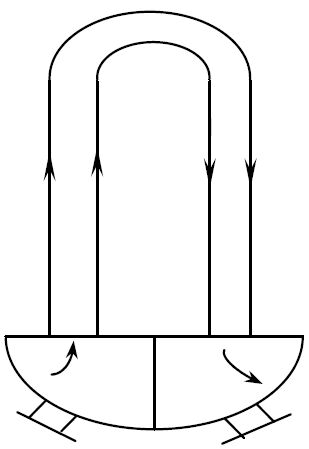
\includegraphics[width=0.3\textwidth]{一回路侧水力计算简图.jpg}
              \caption{一回路侧水力计算简图}
              \label{Fig.1}
          \end{figure}
    \item 局部阻力:$ ( \bigtriangleup P_l) $:
          \begin{equation*}
              \bigtriangleup P_l = \xi \frac{\rho_1u_{1}^{2}}{2}
          \end{equation*}
          式中:$ \xi $—局部阻力系数。$ \xi $ 值主要取决于通道的结构型式,通过实验求得,属于经验数据。
          \par 一回路侧总的局部阻力:
          \begin{equation*}
              \Delta P=\Delta P_{A}+\Delta P_{B}+\Delta P_{C}+\Delta P_{D}+\Delta P_{E}+\Delta P_{F}+\Delta P_{G}
          \end{equation*}
          其中:
          \begin{itemize}
              \item 由进口管至进口水室,通道截然突然扩大的局部阻力—$ \Delta P_A $
                    \begin{equation*}
                        \Delta P_{A}=\xi_{A} \cdot \frac{\rho_{A} \cdot u_{A}^{2}}{2}
                    \end{equation*}
              \item 在进口水室内转弯的局部阻力—$ \Delta P_B $
                    \begin{equation*}
                        \Delta P_{B}=\xi_{B} \cdot \frac{\rho_{B} \cdot u_{B}^{2}}{2}
                    \end{equation*}
              \item 由进口水室至传热管束,通道截面突然缩少的局部阻力—$ \Delta P_C $
                    \begin{equation*}
                        \Delta P_{C}=\xi_{C} \cdot \frac{\rho_{C} \cdot u_{C}^{2}}{2}
                    \end{equation*}
              \item 在$ U $型管弯头内转弯$ 180° $的局部阻力—$\Delta P_D$
                    \begin{equation*}
                        \Delta P_{D}=\xi_{D} \cdot \frac{\rho_{D} \cdot u_{D}^{2}}{2}
                    \end{equation*}
              \item 由传热管束至出口水室,通道截面突然扩大的局部阻力—$ \Delta P_E $
                    \begin{equation*}
                        \Delta P_{E}=\xi_{E} \cdot \frac{\rho_{E} \cdot u_{E}^{2}}{2}
                    \end{equation*}
              \item 在出口水室内转弯的局部阻力—$ \Delta P_F $
                    \begin{equation*}
                        \Delta P_{F}=\xi_{F} \cdot \frac{\rho_{F} \cdot u_{F}^{2}}{2}
                    \end{equation*}
              \item 由出口水室至出口接管,通道截面突然缩小的局部阻力—$ \Delta P_G $
                    \begin{equation*}
                        \Delta P_{G}=\xi_{G} \cdot \frac{\rho_{G} \cdot u_{G}^{2}}{2}
                    \end{equation*}
          \end{itemize}
          一回路侧的水阻力:$ \Delta P_H = \Delta P_f + \Delta P_l $
          \par 考虑贮备系数。其值为计算阻力的$10\%$
          \par 因此:$ \Delta P = 1.1 \Delta P_H $
\end{enumerate}

\subsubsection{二回路侧循环倍率的计算}
在设计中,常用二分法来确定循环倍率$ C_R $值和循环速度$ u_o $值。即先假定几个不同的循环倍率$ C_{R1} $、$ C_{R2} $、$ C_{R3} \cdots$值。分别计算其运动压头$ P_{m} $和总阻力$ \Delta P $,通过二分法直到误差在一定范围内,即为稳定工况时的$ C_{R} $值,同时也可求出$ u_{o} $值。
\begin{figure}[H]
    \centering
    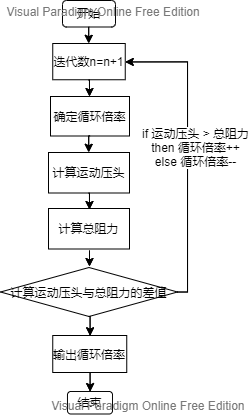
\includegraphics[width=0.7\textwidth]{用二分法计算循环倍率的程序框图.png}
    \caption{用二分法计算循环倍率的程序框图}
    \label{Fig.2}
\end{figure}
\begin{enumerate}
    \item 运动压头$ P_m $的计算:
          \begin{equation*}
              P_{m}=\left(\rho_{l}-\rho_{g}\right) g \varphi H_{r}
          \end{equation*}
          \begin{align*}
              \text{式中:} & H_r \text{—上升空间含汽段高度;}                         \\
                            & \rho_{l},\rho_{g} \text{—分别表示饱和水和饱和汽的密度;} \\
                            & \varphi \text{—表示上升空间平均截面含汽率。}
          \end{align*}
    \item 水循环总阻力$ \Delta P $的计算:
          \begin{align*}
               & \text{总阻力} \Delta P = \Delta P_d + \Delta P_r +\Delta P_s                                                         \\
               & \text{其中:} \Delta P_d \text{、} \Delta P_r \text{和}\Delta P_s \text{—分别表示下降空间、上升空间和分离器的阻力。} \\
               & \text{一般} \Delta P_d \approx 10\% \Delta P \text{,} \Delta P_s 由实验确定                                         \\
               & \text{而} \Delta P_{r}=\Delta P_{f}+\Delta P_{l}+\Delta P_{b}+\Delta P_{a}
          \end{align*}
          式中: $ \Delta P_{f} $ ,$ \Delta P_{l} $ ,$ \Delta P_{b} $ ,和 $ \Delta P_{a} $分别表示摩擦阻力、局部阻力、弯头区阻力和加速度阻力,可按相应的公式进行计算。
\end{enumerate}


\subsection{蒸汽发生器的强度计算}
主要内容有:
\begin{enumerate}
    \item 传热管的强度计算
    \item 筒体的强度计算
    \item 封头的强度计算
    \item 管板的强度计算
\end{enumerate}

\subsubsection{传热管的强度计算}
计算管壁厚度:
\begin{equation*}
    S^{\prime}=\frac{P_{\text {设 }} \cdot d_{0}}{200[\sigma]+0.8 P_{\text {设 }}} \cdot \varphi \cdot \phi_{R}
\end{equation*}
\begin{align*}
    \text{式中:} & P_{\text{设}} \text{—设计压力} (kg/cm^2)               \\
                  & d_o \text{—管子外径} (mm)                              \\
                  & [\sigma] \text{—许用应力}                              \\
                  & \varphi \text{—负公差修正系数,一般取} \varphi = 1.102 \\
                  & \phi_R \text{—弯曲减薄系数}                            \\
                  & \phi_{R}=1+\frac{d_{o}}{4 R}                           \\
                  & \text{式中:R—弯曲半径,取最小节圆半径。}
\end{align*}

\subsubsection{筒体的强度计算}
计算筒体厚度
\begin{equation*}
    S^{\prime}=\frac{P_{\text {设}} \cdot D_{i}}{200[\sigma]-1 \cdot 2 P_{\text {设}}} (mm)
\end{equation*}
式中:$D_i$—筒体内径$ (mm) $

\subsubsection{封头的强度计算}
计算壁厚
\begin{equation*}
    S^{\prime}=\frac{P_{\text {设 }} \cdot D_{o}}{400[\sigma]+1 \cdot 6 P_{\text {设 }}} (mm)
\end{equation*}
式中:$ D_o $—球型封头外径$ (mm) $

\subsubsection{管板的强度计算}
计算壁厚
\begin{equation*}
    S^{\prime}=\frac{1}{2} \cdot F \cdot D \sqrt{\frac{P_{i z}}{[\sigma]}} (mm)
\end{equation*}
\begin{align*}
    \text{式中:} & F \text{—系数,查TEMA 标准}F=1.04 \\
                  & D \text{—水压部分直径} (mm)
\end{align*}

\subsection{蒸汽发生器的结构设计}
主要完成下列工作:
\begin{enumerate}
    \item 管束组件的结构设计
    \item 衬筒的结构设计
    \item 下筒体结构设计
    \item 管板
    \item 分离器组件
    \item 给水管装置
    \item 排污装置
\end{enumerate}

\subsubsection{管束组件的结构设计}
确定流程数,完成传热管的排列,确定管束直径及高度,最佳高-径比一般取为3;确定管子的固定支撑,确定隔板的数目和结构。

\subsubsection{衬筒的结构设计}
确定衬筒的几何形状和尺寸。
\par 衬筒内径:$ D_{w i}=D_{\text {管束 }}+2 \delta_{t} $
\par 式中:$ \delta_t $为装配间隙,约$ 10 \sim 20 mm $。
\par 衬筒外径:$ D_{w o}=D_{w i}+2 \delta $
\par 式中:$ \delta $为衬筒壁厚,约$ 12 mm $。

\subsubsection{下筒体结构设计}
下筒体内径 $ D_{i, \text{下}}=D_{w o}+2 B $
\par 式中:$ B $为下降流道宽度,取为$ 88 mm $。

\subsubsection{管板}
确定开孔数及有关几何尺寸,确定堆焊层与筒体的连接。

\subsubsection{分离器组件}
采用三级汽水分离方式,但不做详细设计,其相应于循环倍率为$ 3,4,5 $时的流动阻力人为设定为$ 12600Pa,14900Pa,17090Pa $。
\subsubsection{给水管装置}
确定给水管的结构,布置及有关几何尺寸。

\subsubsection{排污装置}
确定排污管的结构、布置及有关几何尺寸。

\section{结论与评价}
\subsection{结论}

\subsection{评价}
按照设计要求,本次蒸汽发生器的设计完成了结构设计、热力计算、水动力计算、强度计算,但由于设计者经验上的不足和时间有限等原因,所设计的蒸汽发生器并不是十分满足要求。首先是“高径比”比较小,使得汽水的重力分离不能很好的起到不用,造成这一结果的原因可能是结构参数设计的不够合理。另外,一些经验值的选定不够合理,这主要是由于阅读的文献资料不足。当然,还有很多不尽人意之处,就不在这里赘述了,望读者见谅。





\newpage
\bibliographystyle{plain}
\bibliography{ref/ref.bib}
\thispagestyle{empty}

\pagenumbering{roman}
\setcounter{page}{1}
\begin{appendices}
	\newpage
	\section{附录1 蒸汽发生器热力计算表}
	\begin{table}[H]
    \centering
    \caption{热平衡}
    \scalebox{1.4}{
        \begin{tabular}{|c|c|c|c|c|c|}
            \hline
            序号 & 项目             & 符号           & 单位      & 公式及来源                                                                                     & 数值    \\ \hline
            1    & 一回路放热量     & $ Q $          & $ kW $    & 给定                                                                                           & 2312.11 \\ \hline
            2    & 一回路工作压力   & $ p_1 $        & $ Pa $    & 给定                                                                                           & 15.0    \\ \hline
            3    & 一回路水进口温度 & $ t_{1}^{'} $  & $ ^oC $   & 给定                                                                                           & 310     \\ \hline
            4    & 一回路水出口温度 & $ t_{1}^{''} $ & $ ^oC $   & 给定                                                                                           & 290     \\ \hline
            5    & 一回路水平均温度 & $ t_a $        & $ ^oC $   & $ \frac{1}{2} (t_{1}^{'} + t_{1}^{''}) $                                                       & 300     \\ \hline
            6    & 一回路水进口焓   & $ i_{1}^{'} $  & $ kJ/kg $ & 查表                                                                                           & 1369.04 \\ \hline
            7    & 一回路水出口焓   & $ i_{1}^{''} $ & $ kJ/kg $ & 查表                                                                                           & 1285.82 \\ \hline
            8    & 蒸发器热效率     & $ \eta  $      &           & 给定                                                                                           & 0.99    \\ \hline
            9    & 一回路水流量     & $ G_1 $        & $ kg/s $  & $ \mathrm{Q} / \eta \cdot\left(\mathrm{i}_{1}^{\prime}-\mathrm{i}_{1}^{\prime \prime}\right) $ & 2118.94 \\ \hline
            10   & 二回路工作压力   & $ p_s $        & $ Pa $    & 给定                                                                                           & 5       \\ \hline
            11   & 二回路饱和温度   & $ t_s $        & $ ^oC $   & 查表                                                                                           & 264.0   \\ \hline
            12   & 二回路水饱和焓   & $ i_s $        & $ kJ/kg $ & 查表                                                                                           & 1155.14 \\ \hline
            13   & 二回路给水温度   & $ t_f $        & $ ^oC $   & 给定                                                                                           & 220     \\ \hline
            14   & 二回路给水焓     & $ i_f $        & $ kJ/kg $ & 查表                                                                                           & 944.88  \\ \hline
            15   & 汽化潜热         & $ r $          & $ kJ/kg $ & 查表                                                                                           & 1639.04 \\ \hline
            16   & 蒸汽干度         & $ x $          &           & 给定                                                                                           & 0.99    \\ \hline
            17   & 排放系数         & $ C_s $        &           & 给定                                                                                           & 0.01    \\ \hline
            18   & 二回路蒸汽产量   & $ D $          & $ kg/s $  & $ \frac{Q}{r x+1.01\left(i_{s}-i_{f}\right)} $                                                 & 126     \\ \hline
            19   & 二回路排污量     & $ D_{bd} $     & $ kg/s $  & $ C_s D $                                                                                      & 1.26    \\ \hline
        \end{tabular}
    }
\end{table}

\newpage
\begin{table}[H]
    \centering
    \caption{传热计算}
    \scalebox{1.1}{
        \begin{tabular}{|c|c|c|c|c|c|}
            \hline
            序号 & 项目             & 符号                & 单位      & 公式及来源                                                                                         & 数值  \\ \hline
            20   & 传热管外径       & $ d_o $             & $ kW $    & 选定                                                                                               & 0.022 \\ \hline
            21   & 传热管内径       & $ d_i $             & $ Pa $    & 选定                                                                                               &       \\ \hline
            22   & 单管流通面积     & $ a $               & $ ^oC $   & $ \frac{1}{4} \pi d_{i}^{2} $                                                                      &       \\ \hline
            23   & U 型管数目       & $ n $               & $ ^oC $   & 结构设计定                                                                                         &       \\ \hline
            24   & 一回路流通面积   & $ A $               & $ ^oC $   & $ n \cdot a $                                                                                      &       \\ \hline
            25   & 一回路水平均比容 & $ \overline{v_1}  $ & $ kJ/kg $ & 查表                                                                                               &       \\ \hline
            26   & 一回路水流速     & $ u_1 $             & $ kJ/kg $ & $ G_1 \overline{v_1} / A $                                                                         &       \\ \hline
            27   & 一回路水导热系数 & $ \lambda_1  $      &           & 查表                                                                                               &       \\ \hline
            28   & 一回路水动力粘度 & $ \eta_1 $          & $ kg/s $  & 查表                                                                                               &       \\ \hline
            29   & 一回路水普朗特数 & $ Pr_f $            & $ Pa $    & 查表                                                                                               &       \\ \hline
            30   & 一回路水雷诺数   & $ Re_f $            & $ ^oC $   & $ \mathrm{u}_{1} \mathrm{~d}_{\mathrm{i}} / \eta_{1} \bar{v}_{1} $                                 &       \\ \hline
            31   & 一回路侧放热系数 & $ \alpha_1 $        & $ kJ/kg $ & $ 0.023 \frac{\lambda_{1}}{d_{i}} \operatorname{Re}_{f}^{0.8} \operatorname{Pr}_{f}^{0.4} $        &       \\ \hline
            32   & 传热管导热系数   & $ \lambda_w $       & $ ^oC $   & 给定                                                                                               &       \\ \hline
            33   & 传热管壁热阻     & $ R_w $             & $ kJ/kg $ & $ R_{W}=\frac{d_{o}}{2 \lambda_{w}} \ln \frac{d_{o}}{d_{i}} $                                      &       \\ \hline
            34   & 污垢热阻         & $ R_f $             & $ kJ/kg $ & 按Inconel—600 选定                                                                                 &       \\ \hline
            35   & 二回路侧放热系数 & $ \alpha_2 $        &           & $ \alpha_{2}=0.557 p_{s}^{0.15} q^{0.7} $                                                          &       \\ \hline
            36   & 传热系数         & $ k $               &           & $ \frac{1}{k}=\frac{d_{o}}{d_{i}} \cdot \frac{1}{\alpha_{i}}+R_{w}+\frac{1}{\alpha_{0}}+R_{f} $    &       \\ \hline
            37   & 大端温差         & $ \Delta t_{max} $  & $ kg/s $  & $ t_{1}^{'} - T_s $                                                                                &       \\ \hline
            38   & 小端温差         & $ \Delta t_{min} $  & $ kg/s $  & $ t_{1}^{''} - T_s $                                                                               &       \\ \hline
            39   & 对数平均温差     & $ \Delta t_{ln} $   &           & $ \frac{\Delta t_{\max }-\Delta t_{\min }}{\ln \left(\Delta t_{\max } / \Delta t_{\min }\right)} $ &       \\ \hline
            40   & 热负荷           & $ q $               &           & $ q \cdot \Delta t_{in}$                                                                           &       \\ \hline
            41   & 计算传热面积     & $ F $               &           & $ Q/(10^{-3}q) $                                                                                   &       \\ \hline
            42   & 传热裕度系数     &                     &           & 选定                                                                                               &       \\ \hline
            43   & 设计传热面积     & $ F_{\text{设}} $   & $ m^2 $   & $ C \cdot F $                                                                                      &       \\ \hline
        \end{tabular}
    }
\end{table}

\newpage
\begin{table}[H]
    \centering
    \caption{管束结构}
    \scalebox{1.1}{
        \begin{tabular}{|c|c|c|c|c|c|}
            \hline
            序号 & 项目               & 符号              & 单位  & 公式及来源                                                      & 数值 \\ \hline
            1    & 传热管总长         & $ L_{\text{总}} $ & $ m $ & $ F_{\text{设}} / \pi d_o $                                     &      \\ \hline
            2    & 排列方式           &                   &       & 正方形                                                          &      \\ \hline
            3    & 节 距              & $ t $             & $ m $ & 选定                                                            &      \\ \hline
            4    & 最小U 型管节园直径 & $ D_{\text{节}} $ & $ m $ & $ 4t $                                                          &      \\ \hline
            5    & 实际布管数         & $ n $             & 根    & 结构设计定                                                      &      \\ \hline
            6    & 管束直径           & $ D_{tb} $        & $ m $ & 结构设计定                                                      &      \\ \hline
            7    & 弯管总长           & $ L_{\text{弯}} $ & $ m $ & 结构设计定                                                      &      \\ \hline
            8    & 直管总长           & $ L_{\text{直}} $ & $ m $ & $ L_{\text{总}} - L_{\text{弯}} $                               &      \\ \hline
            9    & 管束直段高         & $ H_{\text{直}} $ & $ m $ & $ L_{\text{直}} / 2n$                                           &      \\ \hline
            10   & 管束弯段高         & $ H_{\text{弯}} $ & $ m $ & $ R_{max} $                                                     &      \\ \hline
            11   & 管束总高           & $ H_{tb} $        & $ m $ & $ H_{\text{直}} + H_{\text{弯}} $                               &      \\ \hline
            12   & 传热管实际平均长度 & $ l $             & $ m $ & $ (\mathrm{L}_\text { 总 } / \mathrm{n})+2 \text { 管板厚 } $   &      \\ \hline
            13   & 最长管子长         & $ l_{max} $       & $ m $ & $ \pi R_{\max }+2 \mathrm{H}_{\text {直 }}+2 \text { 管板厚 } $ &      \\ \hline
            14   & 最短管子长         & $ l_{min} $       & $ m $ & $ \pi R_{\min }+2 \mathrm{H}_{\text {直 }}+2 \text { 管板厚 } $ &      \\ \hline
        \end{tabular}
    }
\end{table}

\newpage
\begin{table}[H]
    \centering
    \caption{主要管道内径}
    \scalebox{1.4}{
        \begin{tabular}{|c|c|c|c|c|c|}
            \hline
            序号 & 项目           & 符号               & 单位       & 公式及来源                                           & 数值 \\ \hline
            1    & 冷却剂平均比容 & $ \overline{v_1} $ & $ m^3/kg $ & 查表                                                 &      \\ \hline
            2    & 主管道计算流速 & $ u_{10}^{'} $     & $ m/s $    & 选取:$ 8 \sim 12 m/s $                              &      \\ \hline
            3    & 主管道计算内径 & $ d_{1i}^{'} $     & $ m $      & $ \sqrt{4 G_{1} \bar{v}_{1} / \pi u_{10}^{\prime}} $ &      \\ \hline
            4    & 主管道设计内径 & $ d_{1i} $         & $ m $      & 选取                                                 &      \\ \hline
            5    & 主管道设计流速 & $ u_{10} $         & $ m/s $    & $ 4 G_{1} \bar{v}_{1} / \pi d_{1 i}^{2} $            &      \\ \hline
            6    & 新蒸汽比容     & $ v_2 $            & $ m^3/kg $ & $ v^{\prime \prime} x+v^{\prime}(1-x) $              &      \\ \hline
            7    & 蒸汽管计算流速 & $ u_{2}^{'} $      & $ m/s $    & 选取:$ 30~40 m/s $                                  &      \\ \hline
            8    & 蒸汽管计算内径 & $ d_{2i}^{'} $     & $ m $      & $ \sqrt{4 G_{2} \bar{v}_{2} / \pi u_{2}^{\prime}} $  &      \\ \hline
            9    & 蒸汽管设计内径 & $ d_{2i} $         & $ m $      & 选取                                                 &      \\ \hline
            10   & 蒸汽管设计流速 & $ u_2 $            & $ m/s $    & $ 4 G_{2} v_{2} / \pi d_{2 i}^{2} $                  &      \\ \hline
            11   & 二回路给水比容 & $ v_3 $            & $ m^3/kg $ & 查表                                                 &      \\ \hline
            12   & 给水管计算流速 & $ u_{3}^{'} $      & $ m/s $    & 选取:$ 2 \sim 5 m/s $                               &      \\ \hline
            13   & 给水管计算内径 & $ d_{3i}^{'} $     & $ m $      & $ \sqrt{4 G_{3} v_{3} / \pi u_{3}^{\prime}} $        &      \\ \hline
            14   & 给水管设计内径 & $ d_{3i} $         & $ m $      & 选取                                                 &      \\ \hline
            15   & 给水管设计流速 & $ u_3 $            & $ m/s $    & $ 4 G_{3} v_{3} / \pi \cdot d_{3 i}^{2} $            &      \\ \hline
        \end{tabular}
    }
\end{table}

	\newpage
	\section{附录2 蒸汽发生器水力计算表}
	\subsection{一回路水阻力计算}

\begin{table}[H]
    \centering
    \caption{U 型管内摩擦阻力计算}
    \scalebox{1.3}{
        \begin{tabular}{|c|c|c|c|c|c|}
            \hline
            序号 & 项目               & 符号               & 单位                                           & 公式及来源                                                                                         & 数值             \\ \hline
            1    & 传热管实际平均长度 & $ l $              & $ m $                                          & 结构设计                                                                                           & 11.38            \\ \hline
            2    & 当量直径           & $ d_i $            & $ m $                                          & 结构设计                                                                                           & 0.0193           \\ \hline
            3    & 一回路水流量       & $ G_1 $            & $ kg/s $                                       & 热工计算定                                                                                         & 2118.94          \\ \hline
            4    & 一回路水平均比容   & $ \overline{v_1} $ & $ m^3/kg $                                     & 查 表                                                                                              & $ 1.38*10^{-3} $ \\ \hline
            5    & 一回路水流速       & $ u_1 $            & $ m/s $                                        & 热工计算定                                                                                         & 5.86             \\ \hline
            6    & 考虑堵管后流速     & $ u_{1}^{'} $      & $ m/s $                                        & $ 1.05u_1 $                                                                                        & 6.153            \\ \hline
            7    & 一回路水雷诺数     & $ Re $             & $ \frac{u_{1}^{'}d_i}{\rho_1 \overline{v_1}} $ & 热工计算定                                                                                         & $ 9.85*10^{-5} $ \\ \hline
            8    & 摩擦阻力系数       & $ \lambda $        &                                                & $ 0.3164Re^{-0.25} $                                                                               & 0.01             \\ \hline
            9    & 平均温度下动力粘度 & $ \eta_{1} $       & $ kg/m \cdot s $                               & 查 表                                                                                              & $ 8.83*10^{-5} $ \\ \hline
            10   & 壁温下动力粘度     & $ \eta_{1}^{'} $   & $ kg/m \cdot s $                               & 按$ \frac{1}{2}(t_a + t_s) $查表                                                                   & $ 9.26*10^{-5} $ \\ \hline
            11   & 温度修正系数       & $ \varphi $        &                                                & $ \left(\eta_{1} / \eta_{1}^{\prime}\right)^{0.14} $                                               & 0.9934           \\ \hline
            12   & 摩擦阻力           & $ \Delta P_f $     & $ Pa $                                         & $ \lambda \cdot \frac{H_{\text {直 }}}{d_{i}} \cdot \frac{u_{1}^{\prime 2}}{\varphi \bar{v}_{1}} $ & 73346.9          \\ \hline
        \end{tabular}
    }
\end{table}

\newpage
\begin{table}[H]
    \centering
    \caption{局部阻力计算}
    \scalebox{1.1}{
        \begin{tabular}{|c|c|c|c|c|c|}
            \hline
            序号 & 项目                & 符号           & 单位       & 公式及来源                                               & 数值    \\ \hline
            13   & 下封头内径          & $ D_1 $        & $ m $      & 结构设计定                                               & 2.26    \\ \hline
            14   & 水室截面积          & $ F_c $        & $ m^2 $    & $ \frac{\pi}{8}D_{1}^{2} $                               & 2       \\ \hline
            15   & 进口管内径          & $ d_{1i} $     & $ m $      & 选定                                                     & 0.62    \\ \hline
            16   & 进口管截面积        & $ A_1 $        & $ m^2 $    & $ \frac{\pi}{4} \cdot d_{1i}^{2} $                       & 0.3     \\ \hline
            17   & 比 值               &                &            & $ A_1/F_c $                                              & 0.15    \\ \hline
            18   & 突扩阻力系数        & $ \xi_1 $      &            & 查表                                                     & 0.7     \\ \hline
            19   & 一回路水入口处比容  & $ v_{1i} $     & $ m^3/kg $ & 查表                                                     & 0.00142 \\ \hline
            20   & 一回路水入口处密度  & $ \rho_{1i} $  & $ kg/m^3 $ & $ 1/v_{1i} $                                             & 703.63  \\ \hline
            21   & 入口管内流速        & $ u_{1i} $     & $ m/s $    & 热工计算定                                               & 9.75    \\ \hline
            22   & 从入口管至水室阻力  & $ \Delta P_1 $ & $ Pa $     & $ \xi_{1} \cdot \frac{u_{1 i}^{2} \cdot \rho_{1 i}}{2} $ & 23411   \\ \hline
            23   & 水室转弯45°阻力系数 & $ \xi_2 $      &            & 查表                                                     & 0.9     \\ \hline
            24   & 水室转弯45°阻力     & $ \Delta P_2 $ & $ Pa $     & $ \xi_{2} \cdot \frac{u_{1 i}^{2} \cdot \rho_{1 i}}{2} $ & 9323.7  \\ \hline
            25   & 传热管流道截面      & $ A $          & $ m^2 $    & 热工计算定                                               & 0.498   \\ \hline
            26   & 考虑有堵管后截面    & $ A^{'} $      & $ m^2 $    & $ A/1.05 $                                               & 0.474   \\ \hline
            27   & 系 数               &                &            & $ A^{'}/F_{c} $                                          & 0.237   \\ \hline
            28   & 传热管入口阻力系数  & $ \xi_3 $      &            & 查表                                                     & 0.5     \\ \hline
            29   & 传热管入口阻力      & $ \Delta P_3 $ & $ Pa $     & $ \xi_{3} \cdot \frac{u_{1 i}^{2} \cdot \rho_{1 i}}{2} $ & 6659.7  \\ \hline
            30   & U型管转180°阻力系数 & $ \xi_4 $      &            & 查表                                                     & 0.5     \\ \hline
            31   & U 型管转180°阻力    & $ \Delta P_4 $ & $ Pa $     & $ \xi_{4} \cdot \frac{u_{1 i}^{2} \cdot \rho_{1 }}{2} $  & 7057.8  \\ \hline
            32   & 传热管出口阻力系数  & $ \xi_5 $      &            & 查表                                                     & 0.6     \\ \hline
            33   & 出口处水比容        & $ v_2 $        & $ m^3/kg $ & 查表                                                     & 0.00134 \\ \hline
            34   & 出口处水密度        & $ \rho_2 $     & $ kg/m^3 $ & $ 1/v_2 $                                                & 745.68  \\ \hline
            35   & 传热管出口阻力      & $ \Delta P_5 $ & $ Pa $     & $ \xi_{5} \cdot \frac{u_{1 i}^{2} \cdot \rho_{2 }}{2} $  & 8469.3  \\ \hline
            36   & 出口管内流速        & $ u_2 $        & $ m/s $    & $ G_1v_2/A_1 $                                           & 9.75    \\ \hline
            37   & 水室转弯阻力系数    & $ \xi_6 $      &            & 查表                                                     & 0.9     \\ \hline
            38   & 水室转弯阻力        & $ \Delta P_6 $ & $ Pa $     & $ \xi_6 \cdot \frac{u_2 \rho_2}{2} $                     & 29966   \\ \hline
            39   & 出口管突缩阻力系数  & $ \xi_7 $      &            & 查表                                                     & 0.44    \\ \hline
            40   & 出口管突缩阻力      & $ \Delta P_7 $ & $ Pa $     & $ \xi_7 \cdot \frac{u_{2}^{2} \rho_2}{2} $               & 15595   \\ \hline
        \end{tabular}
    }
\end{table}

\begin{table}[H]
    \centering
    \caption{总阻力}
    \scalebox{1.1}{
        \begin{tabular}{|c|c|c|c|c|c|}
            \hline
            序号 & 项目     & 符号                     & 单位   & 公式及来源                                   & 数值     \\ \hline
            41   & 总阻力   & $ \Delta P $             & $ Pa $ & $ \Delta P_{f}+\sum_{i=1}^{7} \Delta P_{i} $ & 194607.7 \\ \hline
            42   & 设计阻力 & $ \Delta P_{\text{设}} $ & $ Pa $ & $ 1.1 \Delta P $                             & 214068   \\ \hline
        \end{tabular}
    }
\end{table}

\subsection{二回路水循环阻力计算}

\subsubsection{下降空间阻力}
\begin{table}[H]
    \centering
    \caption{下降空间阻力}
    \scalebox{1.3}{
        \begin{tabular}{|c|c|c|c|c|c|}
            \hline
            序号 & 项目             & 符号           & 单位       & 公式及来源                                                            & 数值             \\ \hline
            1    & 循环倍率         & $ C_R $        &            & 假定                                                                  & 4                \\ \hline
            2    & 给水温度         & $ t_f $        & $ ^oC $    & 给定                                                                  & 220              \\ \hline
            3    & 二回路饱和温度   & $ t_s $        & $ ^oC $    & 查表                                                                  & 264              \\ \hline
            4    & 下降空间水比容   & $ v_d $        & $ m^3/kg $ & 近似取饱和比容                                                        & $ 1.29*10^{-3} $ \\ \hline
            5    & 下降空间水密度   & $ \rho_d $     & $ kg/m^3 $ & $ \frac{1}{v_d} $                                                     & 777.58           \\ \hline
            6    & 入口阻力系数     & $ \xi_{in} $   &            & 选取                                                                  & 1                \\ \hline
            7    & 出口阻力系数     & $ \xi_{out} $  &            & 选取                                                                  & 1                \\ \hline
            8    & 定位装置阻力系数 & $ \xi_f $      &            & 选取                                                                  & 1                \\ \hline
            9    & 下降空间高度     & $ H_0 $        & $ m $      & 结构设计定                                                            & 7.0              \\ \hline
            10   & 套筒外径         & $ D_{w0} $     & $ m $      & 结构设计定                                                            & 2.15             \\ \hline
            11   & 下筒体内径       & $ D_{si} $     & $ m $      & 结构设计定                                                            & 2.33             \\ \hline
            12   & 下降空间当量直径 & $ D_{si} $     & $ m $      & $ D_{si} - D_{wo} $                                                   & 0.18             \\ \hline
            13   & 绝对粗糙度       & $ \Delta $     & $ m $      & 选定                                                                  & $ 1.5*10^{-4} $  \\ \hline
            14   & 摩擦系数         & $ \lambda_d $  &            & $ \frac{1}{(1.74+21g \frac{De}{2 \Delta})^2} $                        & 0.019            \\ \hline
            15   & 下降空间截面积   & $ F_d $        & $ m^2 $    & $ \frac{\pi}{4}(D_{si}^{2}-D_{wo}^{2}) $                              & 0.633            \\ \hline
            16   & 下降空间水流速   & $ u_d $        & $ m/s $    & $ C_R \cdot D \cdot v_d / F_d $                                       & 1.02             \\ \hline
            17   & 下降空间阻力     & $ \Delta P_d $ & $ Pa $     & $ (\lambda \frac{H_o}{De}+\sum \xi)\frac{u_{d}^{2} \cdot \rho_d}{2} $ & 1533.98          \\ \hline
        \end{tabular}
    }
\end{table}

\newpage
\subsubsection{上升空间阻力}
\begin{table}[H]
    \centering
    \caption{摩擦阻力}
    \scalebox{1.0}{
        \begin{tabular}{|c|c|c|c|c|c|}
            \hline
            序号 & 项目                         & 符号                      & 单位       & 公式及来源                                                                                    & 数值             \\ \hline
            1    & 饱和水比容                   & $ v^{'} $                 & $ m^3/kg $ & 查表                                                                                          & $ 1.29*10^{-3} $ \\ \hline
            2    & 饱和水密度                   & $ \rho^{'} $              & $ kg/m^3 $ & $ 1/v^{'} $                                                                                   & 777.61           \\ \hline
            3    & 饱和蒸汽比容                 & $ v^{''} $                & $ m^3/kg $ & 查表                                                                                          & 0.039            \\ \hline
            4    & 饱和蒸汽密度                 & $ \rho^{''} $             & $ kg/m^3 $ & $ 1/v^{'} $                                                                                   & 25.36            \\ \hline
            5    & 套筒内径                     & $ D_{w1} $                & $ m $      & 结构设计定                                                                                    & 2.13             \\ \hline
            6    & 传热管外径                   & $ d_0 $                   & $ m $      & 热工计算定                                                                                    & 0.022            \\ \hline
            7    & 支撑板定位拉杆数量           & $ n^{'} $                 & 根         & 结构设计定                                                                                    & 12               \\ \hline
            8    & 上升空间流通面积             & $ F_u $                   & $ m^2 $    & $ \frac{\pi}{4}[D_{w_1}^{2}-(2n+n^{'})d_{o}^{2}] $                                            & 2.26             \\ \hline
            9    & 上升空间当量直径             & $ de $                    & $ m $      & $ \frac{4F_u}{\pi[D_{wi}+(2n+n^{'})d_o]} $                                                    & 0.037            \\ \hline
            10   & 循环速度                     & $ u_o $                   & $ m/s $    & $ \frac{C_RDv^{'}}{F_u} $                                                                     & 0.288            \\ \hline
            11   & 出口水相折算速度             & $ u_{o2}^{'} $            & $ m/s $    & $ \frac{(C_R - 1)Dv^{'}}{F_u} $                                                               & 0.22             \\ \hline
            12   & 水相平均折算速度             & $ \overline{u_{o}^{'}} $  & $ m/s $    & $ \frac{1}{2}(u_o + u_{o2}^{'}) $                                                             & 0.25             \\ \hline
            13   & 出口汽相折算速度             & $ u_{o2}^{''} $           & $ m/s $    & $ Dv^{''} / F_u $                                                                             & 2.17             \\ \hline
            14   & 汽相平均折算速度             & $ \overline{u_{o}^{''}} $ &            & $ \frac{1}{2}u_{o2}^{''} $                                                                    & 1.09             \\ \hline
            15   & 水相运动粘度                 & $ v_1 $                   & $ m^2/s $  & 查表                                                                                          & $ 1.28*10^{-7} $ \\ \hline
            16   & 汽相运动粘度                 & $ v_g $                   & $ m^2/s $  & 查表                                                                                          & $ 7.11*10^{-7} $ \\ \hline
            17   & 水相雷诺数                   & $ Re_{lo} $               &            & $ \overline{u_{o}^{'}} de / v_l $                                                             & 72800            \\ \hline
            18   & 汽相雷诺数                   & $ Re_{go} $               &            & $ \overline{u_{o}^{''}} de / v_g $                                                            & 56700            \\ \hline
            19   & 判别流态                     &                           &            & 临界值:$ 1000 $                                                                              & 紊流             \\ \hline
            20   & 管束直段高                   & $ H_s $                   & $ m $      & 结构设计定                                                                                    & 4.46             \\ \hline
            21   & 水相摩阻系数                 & $ \lambda_{lo} $          &            & $ 0.3164Re_{lo}^{-0.25} $                                                                     & 0.019            \\ \hline
            22   & 汽相摩阻系数                 & $ \lambda_{go} $          &            & $ 0.3164Re_{go}^{-0.25} $                                                                     & 0.021            \\ \hline
            23   & 按折算速度计算的水相摩擦阻力 & $ (\Delta P_f)_{lo} $     & $ Pa $     & $ \lambda_{lo} \frac{H_s}{de} \frac{\overline{u_{o}^{'2}} \cdot  \rho^{'}}{2} $               & 52.21            \\ \hline
            24   & 按折算速度计算的汽相摩擦阻力 & $ (\Delta P_f)_{go} $     & $ Pa $     & $ \frac{1}{3} \lambda_{lo} \frac{H_s}{de} \frac{\overline{u_{o}^{''2}} \cdot  \rho^{''}}{2} $ & 12.35            \\ \hline
            25   & 参 量 X                      &                           &            & $ \sqrt{(\Delta P_f)_{lo}/(\Delta P_f)_{go}} $                                                & 2.15             \\ \hline
            26   & $ \Phi_{l}^{2} $             &                           &            & 查图或计算                                                                                    & 10.51            \\ \hline
            27   & $ \Phi_{g}^{2} $             &                           &            & 查图或计算                                                                                    & 48.67            \\ \hline
            28   & 水相摩擦阻力                 & $ (\Delta P_f)_{l} $      & $ Pa $     & $ \Phi_{l}^{2} \cdot (\Delta P_f)_{lo} $                                                      & 601.26           \\ \hline
            29   & 汽相摩擦阻力                 & $ (\Delta P_f)_{g} $      & $ Pa $     & $ \Phi_{g}^{2} \cdot (\Delta P_f)_{go} $                                                      & 601.26           \\ \hline
            30   & 摩擦阻力                     & $ \Delta P_f $            & $ Pa $     & $ [(\Delta P_f)_{l}+(\Delta P_f)_{g}]/2 $                                                     & 601.26           \\ \hline
        \end{tabular}
    }
\end{table}

\newpage
\begin{table}[H]
    \centering
    \caption{局部阻力}
    \scalebox{1.1}{
        \begin{tabular}{|c|c|c|c|c|c|}
            \hline
            序号 & 项目                         & 符号                  & 单位       & 公式及来源                                                               & 数值   \\ \hline
            1    & 支撑板数目                   & $ N $                 & 个         & 结构设计定                                                               & 6      \\ \hline
            2    & 上升流道单元面积             & $ A_u $               & $ mm^{2} $ & 结构设计定                                                               & 670    \\ \hline
            3    & 支撑板单元开孔面积           & $ a_u $               & $ mm^{2} $ & 结构设计定                                                               & 147    \\ \hline
            4    & 面 积 比                     &                       &            & $ a_u / A_u $                                                            & 0.22   \\ \hline
            5    & 局部阻力系数                 & $ \xi_l $             &            & 查 图                                                                    & 40     \\ \hline
            6    & 按折算速度计算的水相局部阻力 & $ (\Delta P_l)_{lo} $ & $ Pa $     & $ N \xi_l \frac{\overline{u_{o}^{'2}} \cdot \rho^{'}}{2} $               & 3023.3 \\ \hline
            7    & 按折算速度计算的汽相局部阻力 & $ (\Delta P_l)_{go} $ & $ Pa $     & $ \frac{1}{3} N \xi_l \frac{\overline{u_{o}^{''2}} \cdot \rho^{''}}{2} $ & 1205.2 \\ \hline
            8    & 参 量$ X $                   &                       &            & $ \sqrt{(\Delta P_l)_{lo}/(\Delta P_l)_{go}} $                           & 1.6    \\ \hline
            9    & 二回路工作压力               & $ p_s $               & $ Pa $     & 给定                                                                     & 5      \\ \hline
            10   & 临界压力                     & $ p_c $               & $ Pa $     & 查水蒸汽表                                                               & 22.06  \\ \hline
            11   & 参数$ Z_R $                  &                       &            & $ (0.19+0.92 \frac{p_s}{p_c})^{-1} $                                     & 2.51   \\ \hline
            12   & 参数$ K $                    &                       &            & $ Z_R + \frac{1}{Z_R} $                                                  & 2.91   \\ \hline
            13   & $ \Phi_{l}^{2} $             &                       &            & $ 1 + \frac{K}{X} + \frac{1}{X^{2}} $                                    & 3.24   \\ \hline
            14   & $ \Phi_{g}^{2} $             &                       &            & $ 1+KX + X^{2} $                                                         & 12.26  \\ \hline
            15   & 水相局部阻力                 & $ (\Delta P_l)_{l} $  & $ Pa $     & $ \Phi_{l}^{2} \cdot (\Delta P_l)_{lo} $                                 & 9795.5 \\ \hline
            16   & 汽相局部阻力                 & $ (\Delta P_l)_{g} $  & $ Pa $     & $ \Phi_{g}^{2} \cdot (\Delta P_l)_{go} $                                 & 9749.9 \\ \hline
            17   & 局部阻力                     & $ \Delta P_l $        & $ Pa $     & $ [ (\Delta P_l)_{l} + (\Delta P_l)_{g} ] / 2 $                          & 9749.9 \\ \hline
        \end{tabular}
    }
\end{table}

\newpage
\begin{table}[H]
    \centering
    \caption{弯管区阻力}
    \scalebox{1.1}{
        \begin{tabular}{|c|c|c|c|c|c|}
            \hline
            序号 & 项目                 & 符号                  & 单位  & 公式及来源                                                                                            & 数值    \\ \hline
            1    & 管束弯头最大节园直径 & $ d_b $               & $ m $ & 结构设计定                                                                                            & 2.1     \\ \hline
            2    & 弯管区重心至园心距离 & $ y_s $               & $ m $ & $ 0.2122d_b $                                                                                         & 0.4456  \\ \hline
            3    & 节 距                & $ t $                 & $ m $ & 结构设计定                                                                                            & 0.0297  \\ \hline
            4    & 计算冲刷排数         & $ N^{'} $             &       & $ \frac{y_s}{t} - 1 $(取整数)                                                                         & 14      \\ \hline
            5    & 系 数                & $ x_1 = x_2 $         &       & $ t/d_o $                                                                                             & 1.35    \\ \hline
            6    & 系 数                & $ n $                 &       & $ 0.43 + \frac{1.13}{x_1} $                                                                           & 1.267   \\ \hline
            7    & 水相雷诺数           & $ Re_{lo} $           &       & $ u_{o2}^{'}de / v_l $                                                                                & 41625   \\ \hline
            8    & 汽相雷诺数           & $ Re_{go} $           &       & $ u_{o2}^{''}de / v_g $                                                                               & 112925  \\ \hline
            9    & 水相磨擦阻力系数     & $ \lambda_{lo} $      &       & $ 4\left[0.044+\frac{0.08 x_{2}}{\left(x_{1}-1\right)^{n}}\right] \mathrm{Re}_{l o}^{-0.15} $         & 0.37    \\ \hline
            10   & 汽相磨擦阻力系数     & $ \lambda_{go} $      &       & $ 4\left[0.044+\frac{0.08 x_{2}}{\left(x_{1}-1\right)^{n}}\right] \mathrm{Re}_{g o}^{-0.15} $         & 0.32    \\ \hline
            11   & 水 相 阻 力          & $ (\Delta P_b)_{lo} $ &       & $ N^{\prime} \lambda_{l o} \cdot \frac{u_{o 2}^{\prime} \rho^{\prime}}{2} $                           & 287.41  \\ \hline
            12   & 汽 相 阻 力          & $ (\Delta P_b)_{go} $ &       & $ \frac{1}{3} N^{\prime} \lambda_{g o} \cdot \frac{u_{o 2}^{\prime \prime} \rho^{\prime \prime}}{2} $ & 40.46   \\ \hline
            13   & 参 量$ X $           &                       &       & $ \sqrt{(\Delta P_b)_{lo / (\Delta P_b)_{go}}} $                                                      & 2.66    \\ \hline
            14   & $ \Phi_{lo}^{2} $    &                       &       & 查图或计算(同摩擦阻力)                                                                                & 8.66    \\ \hline
            15   & $ \Phi_{go}^{2} $    &                       &       & 查图或计算(同摩擦阻力)                                                                                & 56.7    \\ \hline
            16   & 水 相 阻 力          & $ (\Delta P_b)_{l} $  &       & $ \Phi_{lo}^{2} \cdot (\Delta P_b)_{l} $                                                              & 2489.64 \\ \hline
            17   & 汽 相 阻 力          & $ (\Delta P_b)_{g} $  &       & $ \Phi_{go}^{2} \cdot (\Delta P_b)_{g} $                                                              & 2304.5  \\ \hline
            18   & 弯 管 区 阻 力       & $ \Delta P_b $        &       & $ [(\Delta P_b)_{l} + (\Delta P_b)_{g}] / 2 $                                                         & 2397.1  \\ \hline
        \end{tabular}
    }
\end{table}

\begin{table}[H]
    \centering
    \caption{加速阻力}
    \scalebox{1.2}{
        \begin{tabular}{|c|c|c|c|c|c|}
            \hline
            序号 & 项目               & 符号           & 单位          & 公式及来源                                                                                                 & 数值   \\ \hline
            1    & 管束出口质量含汽率 & $ x_2 $        &               & $ 1/C_R $                                                                                                  & 0.333  \\ \hline
            2    & 管束出口体积含汽率 & $ \beta_2 $    &               & $ \frac{x_{2} / \rho^{\prime \prime}}{x_{2} / \rho^{\prime \prime}+\left(1-x_{2}\right) / \rho^{\prime}} $ & 0.939  \\ \hline
            3    & 系数               & $ C $          &               & $ 0.833 + 0.05 \ln(\frac{p_s}{10^{6}}) $                                                                   & 0.887  \\ \hline
            4    & 管束出口截面含汽率 & $ \phi_2 $     &               & $ C \beta_2 $                                                                                              & 0.833  \\ \hline
            5    & 质量流速           & $ \dot{G} $    & $ kg/m^{2}s $ & $ u_o \rho^{'} $                                                                                           & 167.78 \\ \hline
            6    & 加速阻力           & $ \Delta p_a $ & $ Pa $        & $ \dot{G}^{2}\left[\begin{array}{l} \frac{\left(1-x_{2}\right)^{2}}{\rho^{\prime}\left(1-\varphi_{2}\right)}+\frac{x_{2}^{2}}{\rho^{\prime \prime} \varphi_{2}} \\ -\frac{1}{\rho^{\prime}} \end{array}\right] $                                                      & 208.1  \\ \hline
        \end{tabular}
    }
\end{table}

\begin{table}[H]
    \centering
    \caption{流量分配孔阻力}
    \scalebox{1.5}{
        \begin{tabular}{|c|c|c|c|c|c|}
            \hline
            序号 & 项目         & 符号           & 单位       & 公式及来源                                  & 数值  \\ \hline
            1    & 单 元 面 积  & $ A_{u}^{'} $  & $ mm^{2} $ & 结构设计定                                  & 533   \\ \hline
            2    & 单元开孔面积 & $ a_{u}^{'} $  & $ mm^{2} $ & 结构设计定                                  & 216   \\ \hline
            3    & 系 数        &                &            & $ a_{u}^{\prime} / A_{u}^{\prime} $         & 0.405 \\ \hline
            4    & 阻 力 系 数  & $ \xi_h $      &            & 查文献                                      & 8     \\ \hline
            5    & 孔板局部阻力 & $ \Delta P_h $ & $ Pa $     & $ \xi_h \frac{u_{0}^{2} \rho^{\prime}}{2} $ & 144.8 \\ \hline
        \end{tabular}
    }
\end{table}

\begin{table}[H]
    \centering
    \caption{上升空间阻力}
    \scalebox{1.1}{
        \begin{tabular}{|c|c|c|c|c|c|}
            \hline
            序号 & 项目         & 符号           & 单位   & 公式及来源                                                         & 数值    \\ \hline
            1    & 上开空间阻力 & $ \Delta P_r $ & $ Pa $ & $ \Delta P_f + \Delta P_l + \Delta P_b + \Delta P_a + \Delta P_h $ & 12936.9 \\ \hline
        \end{tabular}
    }
\end{table}

\subsubsection{汽水分离器阻力}

\begin{table}[H]
    \centering
    \caption{汽水分离器阻力}
    \scalebox{1.3}{
        \begin{tabular}{|c|c|c|c|c|c|}
            \hline
            序号 & 项目           & 符号           & 单位   & 公式及来源 & 数值  \\ \hline
            1    & 汽水分离器阻力 & $ \Delta P_s $ & $ Pa $ &            & 12600 \\ \hline
        \end{tabular}
    }
\end{table}

\subsubsection{循环总阻力}

\begin{table}[H]
    \centering
    \caption{循环总阻力}
    \scalebox{1.3}{
        \begin{tabular}{|c|c|c|c|c|c|}
            \hline
            序号 & 项目       & 符号                     & 单位   & 公式及来源                               & 数值    \\ \hline
            1    & 循环总阻力 & $ \Delta P_{\text{总}} $ & $ Pa $ & $ \Delta P_d + \Delta P_r + \Delta P_s $ & 26399.8 \\ \hline
        \end{tabular}
    }
\end{table}

\subsection{运动压头计算}

\begin{table}[H]
    \centering
    \caption{予热段高度计算}
    \scalebox{1.2}{
        \begin{tabular}{|c|c|c|c|c|c|}
            \hline
            序号 & 项目                        & 符号        & 单位                      & 公式及来源                                                                                                                                                               & 数值             \\ \hline
            1    & 循环倍率                    & $ C_R $     &                           & 假 定                                                                                                                                                                    & 3                \\ \hline
            2    & 二回路给水焓                & $ i_f $     & $ J/kg $                  & 查 表                                                                                                                                                                    & 944880           \\ \hline
            3    & 二回路饱和水焓              & $ i_s $     & $ J/kg $                  & 查 表                                                                                                                                                                    & 1155100          \\ \hline
            4    & 液 面 高 度                 & $ H_o $     & $ m $                     & 结构设计定                                                                                                                                                               & 7                \\ \hline
            5    & 下 降 空 间 水 密 度        & $ \rho_d $  & $ kg/m^{3} $              & 取 $ \rho_d = rho^{\prime} $                                                                                                                                             & 777.61           \\ \hline
            6    & 下降空间下端压力            & $ p_{low} $ & $ Pa $                    & $ p_s + g \rho_d H_o $                                                                                                                                                   & 5053304          \\ \hline
            7    & $ p_{low} $压力下的饱和水焓 & $ i_{sl} $  & $ J/kg $                  & 查 表                                                                                                                                                                    & $ 1.159*10^{6} $ \\ \hline
            8    & $ \Delta i / \Delta P $     &             & $ \frac{J}{kg \cdot Pa} $ & $ (i_{sl} - i_{s}) / (p_{low} - p_{s}) $                                                                                                                                 & 0.0711           \\ \hline
            9    & 热负荷                      & $ q $       & $ W/m^{2} $               & 热工计算定                                                                                                                                                               & 203174           \\ \hline
            10   & 循环水量                    & $ G $       & $ kg/s $                  & $ C_R \cdot D $                                                                                                                                                          & 378              \\ \hline
            11   & 予热段高度                  & $ H_p $     & $ m $                     & $ \frac{\frac{i_{s}-i_{f}}{C_{R}}+\frac{\Delta i}{\Delta P}\left(\rho_{d} g H_{o}-\Delta P_{d}\right)}{\frac{2 \pi d_{o} n q}{G}+\frac{\Delta i}{\Delta P} \rho_{d} g} $ & 0.582            \\ \hline
        \end{tabular}
    }
\end{table}

\begin{table}[H]
    \centering
    \caption{运动压头计算}
    \scalebox{1.2}{
        \begin{tabular}{|c|c|c|c|c|c|}
            \hline
            序号 & 项目                       & 符号                   & 单位   & 公式及来源                                                                                                                   & 数值      \\ \hline
            1    & 蒸发段高度                 & $ H_{r1} $             & $ m $  & $ H_{tb} - H_{P} $                                                                                                           & 4.93      \\ \hline
            2    & 管束上方区段高度           & $ H_{r2} $             & $ m $  & $ H_{o} - H_{tb} $                                                                                                           & 1.51      \\ \hline
            3    & 蒸发段平均质量含汽率       & $ \overline{x_1} $     &        & $ x_2 / 2 $                                                                                                                  & 0.17      \\ \hline
            4    & 蒸发段平均体积含汽率       & $ \overline{\beta_1} $ &        & $ \frac{\bar{x}_{1} / \rho^{\prime \prime}}{\bar{x}_{1} / \rho^{\prime \prime}+\left(1-\bar{x}_{1}\right) / \rho^{\prime}} $ & 0.86      \\ \hline
            5    & 蒸发段平均截面含汽率       & $ \overline{\phi_1} $  &        & $ C \overline{\beta_1} $                                                                                                     & 2.58      \\ \hline
            6    & 管束上方区段平均截面含汽率 & $ \overline{\phi_2} $  &        & $ \overline{\phi_2} = \phi_2 $                                                                                               & 0.83      \\ \hline
            7    & 蒸发段运动压头             & $ P_{m1} $             & $ Pa $ & $ (\rho^{'} - \rho^{''})g \overline{\phi_1} H_{r1} $                                                                         & 93705.62  \\ \hline
            8    & 管束上方区段压头           & $ P_{m2} $             & $ Pa $ & $ (\rho^{'} - \rho^{''})g \overline{\phi_2} H_{r2} $                                                                         & 9269.31   \\ \hline
            9    & 运动压头                   & $ P_m $                & $ Pa $ & $ P_{m1} + P_{m2} $                                                                                                          & 102974.93 \\ \hline
        \end{tabular}
    }
\end{table}

	\newpage
	\section{附录3 蒸汽发生器强度计算表}
	\subsection{传热管}

\begin{table}[H]
    \centering
    \caption{传热管}
    \scalebox{1.25}{
        \begin{tabular}{|c|c|c|c|c|c|}
            \hline
            序号 & 项目           & 符号               & 单位          & 公式及来源                                                                  & 数值  \\ \hline
            1    & 设计压力       & $ P_{\text{设}1} $ & $ kg/cm^{2} $ & 选定                                                                        & 191   \\ \hline
            2    & 许用应力       & $ [\sigma] $       & $ kg/mm^{2} $ & 查表                                                                        & 18    \\ \hline
            3    & 管子外径       & $ d_o $            & $ mm $        & 选定                                                                        & 22    \\ \hline
            4    & 直管计算壁厚   & $ S^{''} $         & $ mm $        & $ \frac{P_{\text {设 } 1} \cdot d_{o}}{200[\sigma]+0.8 P_{\text {设 } 1}} $ & 1.12  \\ \hline
            5    & 负公差修正系数 & $ \phi $           &               & 技术条件测定                                                                & 1.102 \\ \hline
            6    & 弯曲减薄系数   & $ \Phi_R $         &               & $ 1 + d_o / 4R $                                                            & 1.093 \\ \hline
            7    & 计算壁厚       & $ S^{'} $          & $ mm $        & $ S^{''} \cdot \phi \cdot \phi_R $                                          & 1.350 \\ \hline
            8    & 设计壁厚       & $ S $              & $ mm $        & 选取                                                                        & 1.40  \\ \hline
        \end{tabular}
    }
\end{table}

\subsection{下筒体}

\begin{table}[H]
    \centering
    \caption{下筒体}
    \scalebox{1.25}{
        \begin{tabular}{|c|c|c|c|c|c|}
            \hline
            序号 & 项目           & 符号                & 单位          & 公式及来源                                                                     & 数值   \\ \hline
            1    & 设计压力       & $ P_{\text{设},2} $ & $ kg/cm^{2} $ & 选定                                                                           & 63.75  \\ \hline
            2    & 许用应力       & $ [\sigma] $        & $ kg/mm^{2} $ & 查表                                                                           & 18     \\ \hline
            3    & 筒体内径       & $ D_{i,\text{下}} $ & $ mm $        & 结构设计定                                                                     & 2264.2 \\ \hline
            4    & 设计壁厚       & $ S^{'} $           & $ mm $        & $ \frac{P_{\text {设 } 2} \cdot D_{i 下}}{200[\sigma]-1.2 P_{\text {设 } 2}} $ & 42.59  \\ \hline
            5    & 设计壁厚       & $ S $               & $ mm $        & 选定                                                                           & 42.6   \\ \hline
            6    & 筒体外径       & $ D_{o,\text{下}} $ & $ mm $        & $ D_{i,\text{下}} + 2S $                                                       & 2415.2 \\ \hline
            7    & 与管板连接壁厚 & $ S_{I} $           & $ mm $        & 选定                                                                           & 50     \\ \hline
        \end{tabular}
    }
\end{table}

\subsection{上筒体}

\begin{table}[H]
    \centering
    \caption{上筒体}
    \scalebox{1.25}{
        \begin{tabular}{|c|c|c|c|c|c|}
            \hline
            序号 & 项目     & 符号                & 单位          & 公式及来源                                                                            & 数值  \\ \hline
            1    & 设计压力 & $ P_{\text{设},2} $ & $ kg/cm^{2} $ & 选定                                                                                  & 63.75 \\ \hline
            2    & 许用应力 & $ [\sigma] $        & $ kg/mm^{2} $ & 查表                                                                                  & 18    \\ \hline
            3    & 筒体内径 & $ D_{i,\text{下}} $ & $ mm $        & 结构设计定                                                                            & 3200  \\ \hline
            4    & 设计壁厚 & $ S^{'} $           & $ mm $        & $ \frac{P_{\text {设 } 2} \cdot D_{i \text{上}}}{200[\sigma]-1.2 P_{\text {设 } 2}} $ & 57.90 \\ \hline
            5    & 设计壁厚 & $ S $               & $ mm $        & 选定                                                                                  & 58    \\ \hline
        \end{tabular}
    }
\end{table}

\subsection{球形下封头}

\begin{table}[H]
    \centering
    \caption{球形下封头}
    \scalebox{1.25}{
        \begin{tabular}{|c|c|c|c|c|c|}
            \hline
            序号 & 项目         & 符号                & 单位          & 公式及来源                                                                    & 数值   \\ \hline
            1    & 设计压力     & $ P_{\text{设},1} $ & $ kg/cm^{2} $ & 选定                                                                          & 191.25 \\ \hline
            2    & 许用应力     & $ [\sigma] $        & $ kg/mm^{2} $ & 查表                                                                          & 14.5   \\ \hline
            3    & 球形封头外径 & $ D_o $             & $ mm $        & 结构设计定                                                                    & 2415.2 \\ \hline
            4    & 计算壁厚     & $ S^{'} $           & $ mm $        & $ \frac{P_{\text {设 } 1} \cdot D_{0}}{400[\sigma] + 1.6 P_{\text {设 } 1}} $ & 74.47  \\ \hline
            5    & 设计壁厚     & $ S $               & $ mm $        & 选取                                                                          & 75.0   \\ \hline
        \end{tabular}
    }
\end{table}

\subsection{管板}

\begin{table}[H]
    \centering
    \caption{管板}
    \scalebox{1.1}{
        \begin{tabular}{|c|c|c|c|c|c|}
            \hline
            序号 & 项目                 & 符号                & 单位          & 公式及来源                                       & 数值   \\ \hline
            1    & 设计压力             & $ P_{\text{设},1} $ & $ kg/cm^{2} $ & 选定                                             & 191.25 \\ \hline
            2    & 许用应力             & $ [\sigma] $        & $ kg/mm^{2} $ & 查表                                             & 1800   \\ \hline
            3    & 承压部分直径         & $ D $               & $ mm $        & 结构设计定                                       & 2124.4 \\ \hline
            4    & 筒体根部壁厚与直径比 &                     &               & $ S/D $                                          & 0.17   \\ \hline
            5    & 系 数                & $ F $               &               & 查TEMA 标准                                      & 1.04   \\ \hline
            6    & 计算壁厚             & $ S^{'} $           & $ mm $        & $ \frac{1}{2} FD \sqrt{P_{\text{设}}/[\sigma]} $ & 356.72 \\ \hline
            7    & 设计壁厚             & $ S $               & $ mm $        & 选取                                             & 360    \\ \hline
            8    & 堆焊层厚度           & $ S^{'} $           & $ mm $        & 选取                                             & 6      \\ \hline
        \end{tabular}
    }
\end{table}

	\newpage
	\section{附图1 蒸发器总图}
	% \begin{figure}[H]
%     \centering
%     \caption{蒸汽发生器图纸}
%     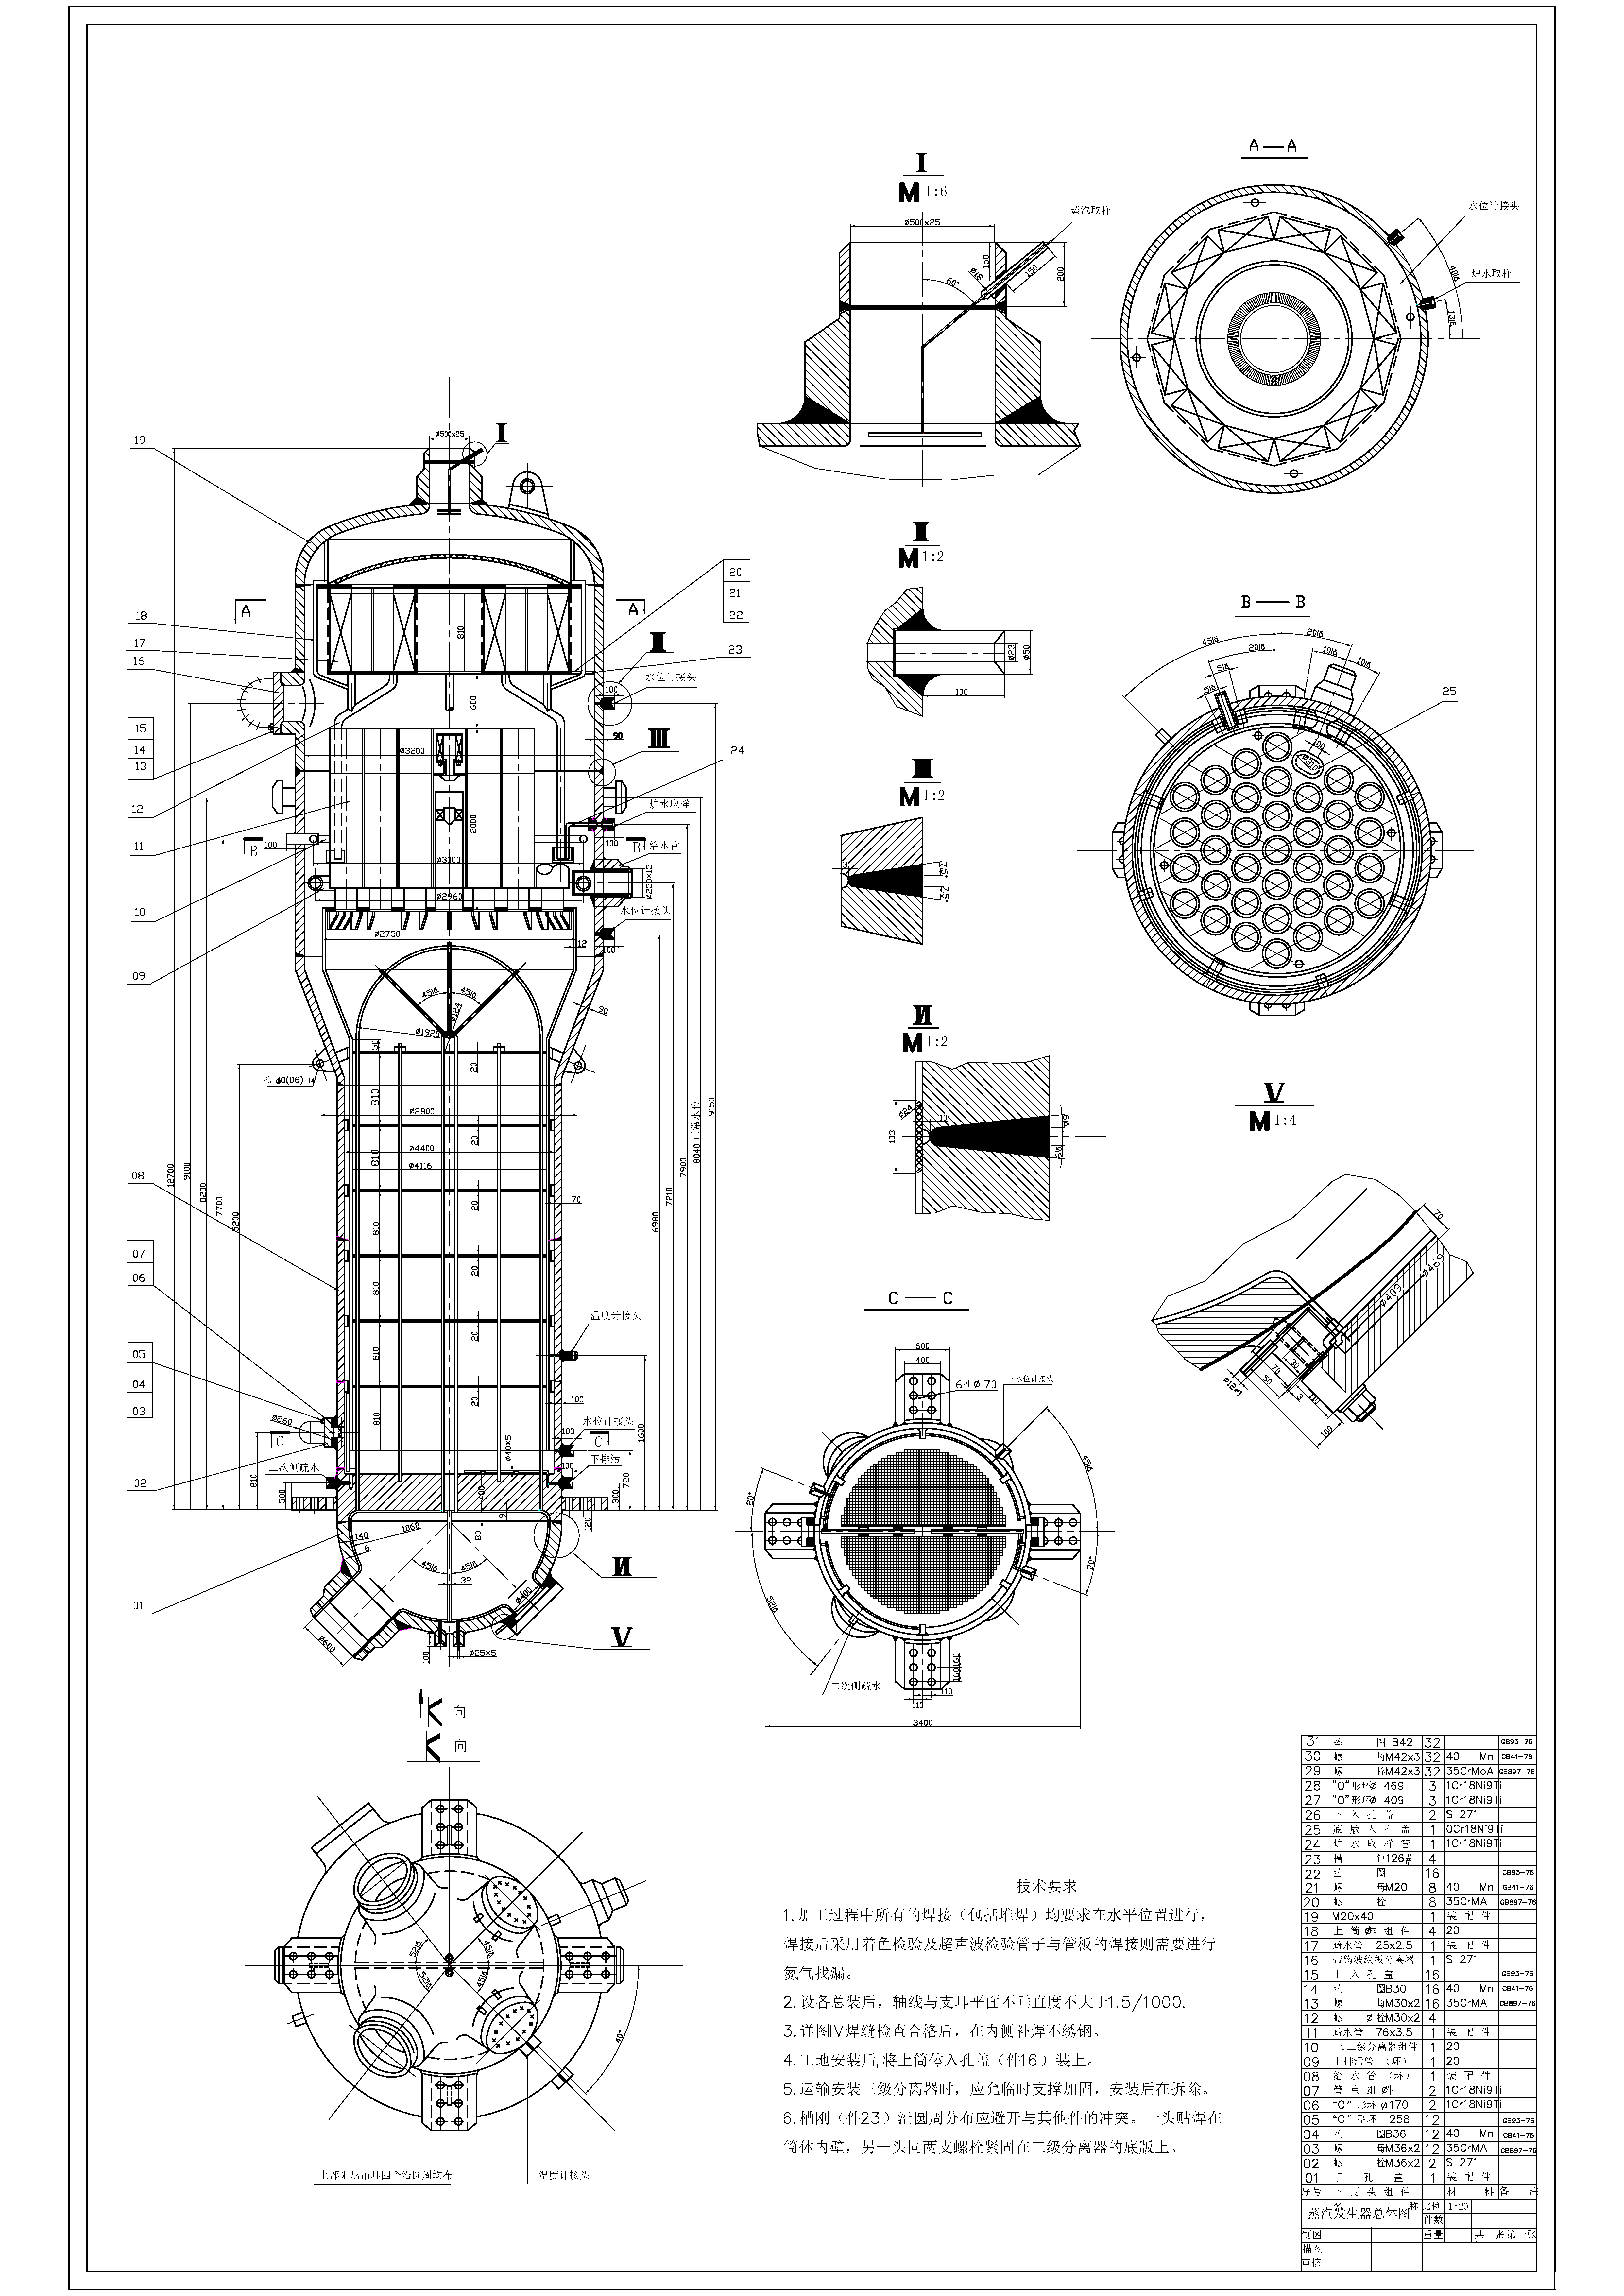
\includegraphics[width=1.0\textwidth]{图纸-蒸汽发生器.pdf}
%     \label{蒸汽发生器图纸}
% \end{figure}
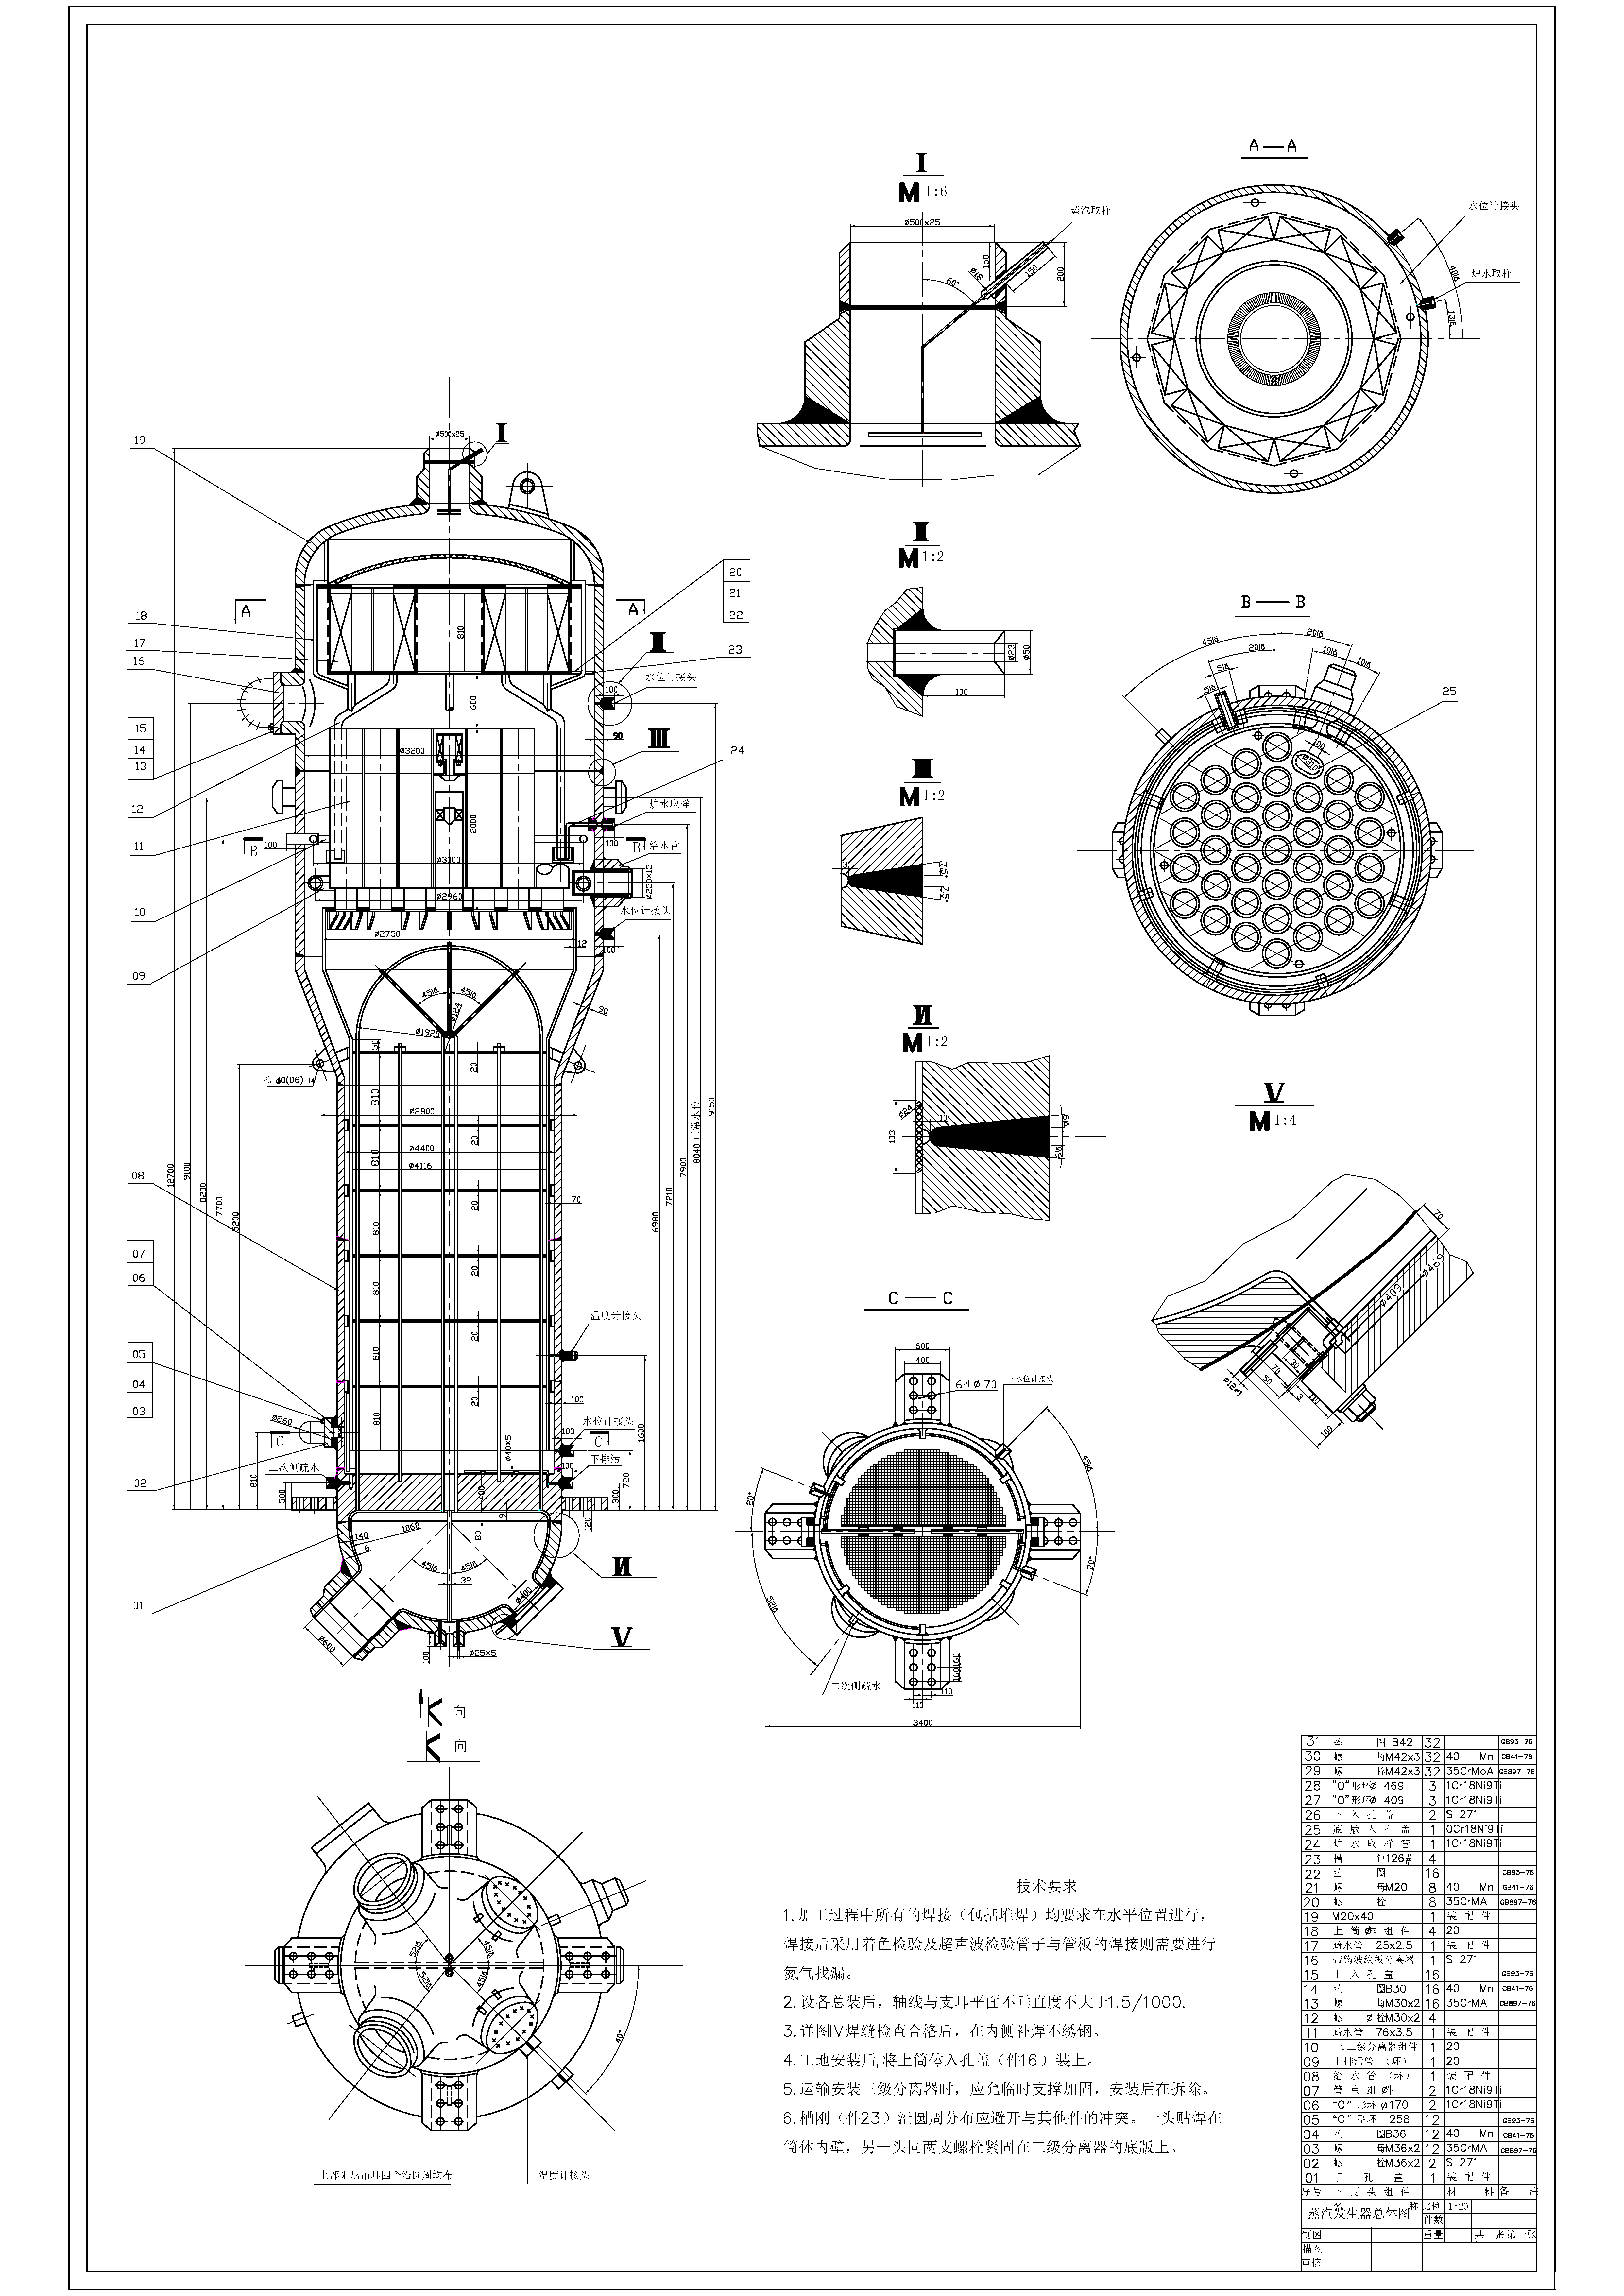
\includegraphics[width=1.0\textwidth]{图纸-蒸汽发生器.pdf}

	% \newpage
	% \section{附图2 蒸发器部件图}
	% \subsection{蒸汽发生器主体}

\begin{figure}[H]
    \centering
    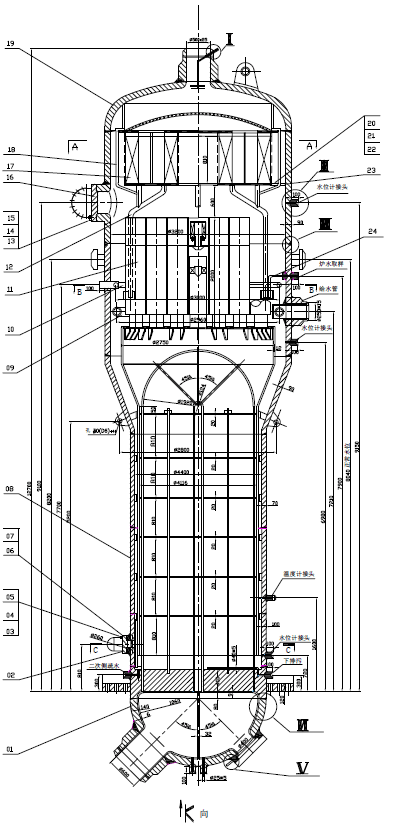
\includegraphics[width=0.3\textwidth]{蒸汽发生器主体.png}
    \caption{蒸汽发生器主体}
    \label{蒸汽发生器主体}
\end{figure}

\subsection{蒸汽发生器俯视图}

\begin{figure}[H]
    \centering
    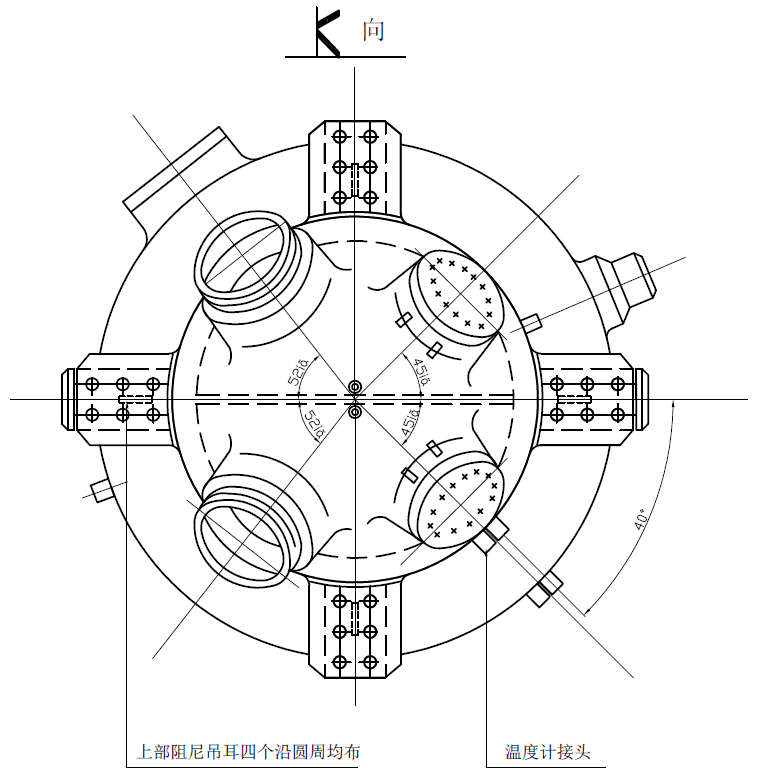
\includegraphics[width=0.5\textwidth]{蒸汽发生器俯视图.png}
    \caption{蒸汽发生器俯视图}
    \label{蒸汽发生器俯视图}
\end{figure}

\subsection{蒸汽发生器顶部剖面}

\begin{figure}[H]
    \centering
    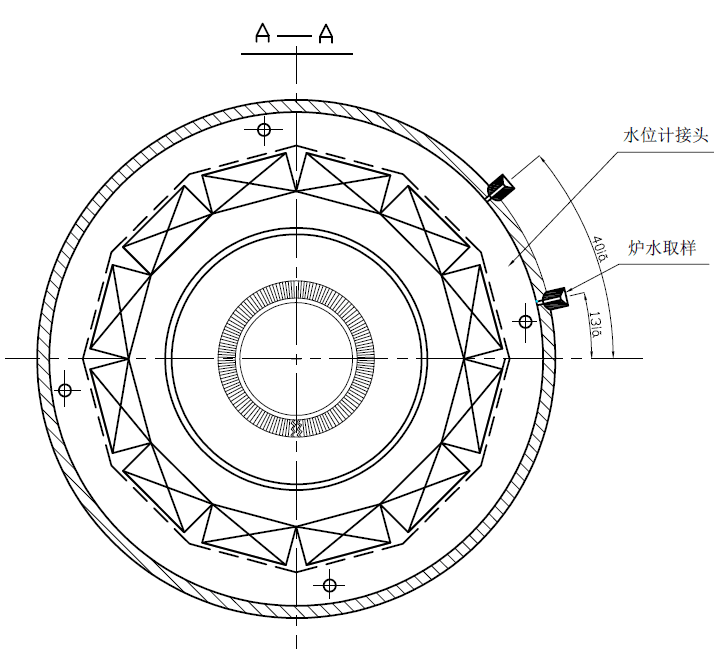
\includegraphics[width=0.6\textwidth]{剖面A.png}
    \caption{蒸汽发生器顶部剖面}
    \label{蒸汽发生器顶部剖面}
\end{figure}

\subsection{蒸汽发生器中部剖面}

\begin{figure}[H]
    \centering
    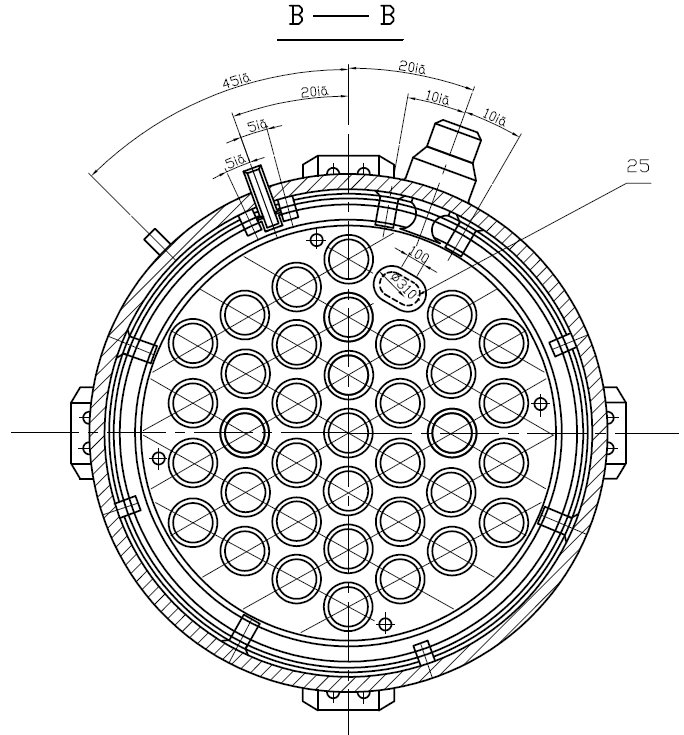
\includegraphics[width=0.6\textwidth]{剖面B.png}
    \caption{蒸汽发生器中部剖面}
    \label{蒸汽发生器中部剖面}
\end{figure}

\subsection{蒸汽发生器底部剖面}

\begin{figure}[H]
    \centering
    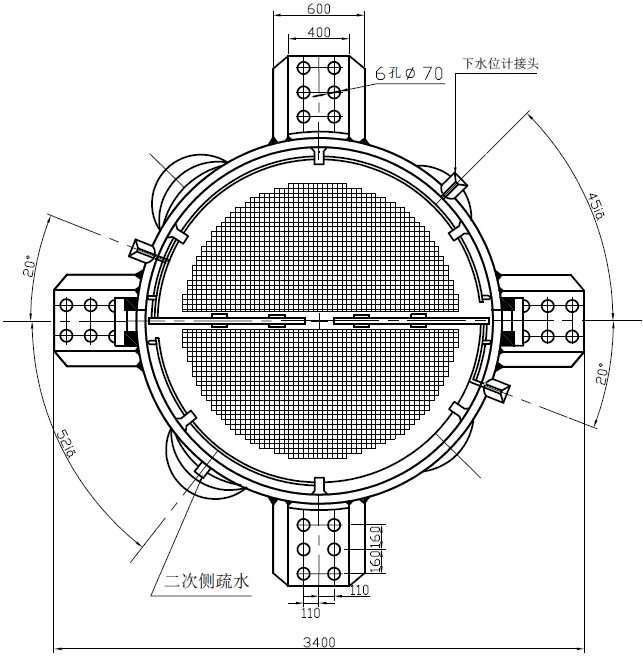
\includegraphics[width=0.6\textwidth]{剖面C.png}
    \caption{蒸汽发生器底部剖面}
    \label{蒸汽发生器底部剖面}
\end{figure}

\subsection{蒸发发生器局部切面}

\begin{figure}[htbp]
    \centering
    \subfigure[蒸汽出口切面]{
        \begin{minipage}[t]{0.25\linewidth}
            \centering
            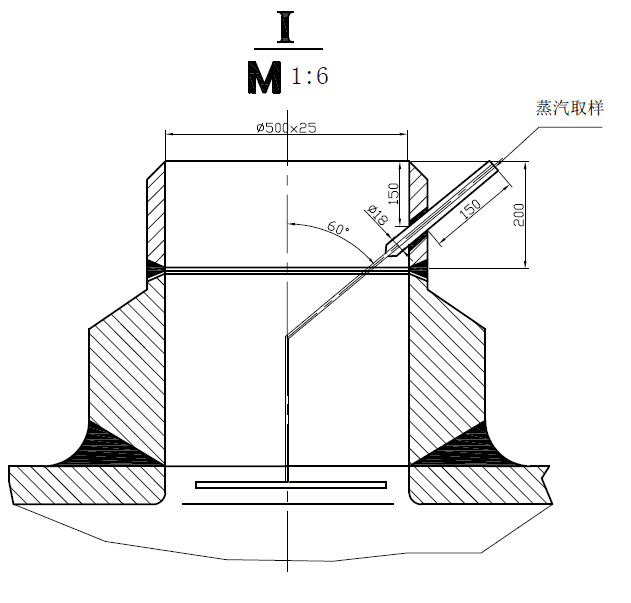
\includegraphics[width=1in]{切面1.png}
            % \caption{fig1}
        \end{minipage}
    }
    \subfigure[水位计接口切面]{
        \begin{minipage}[t]{0.25\linewidth}
            \centering
            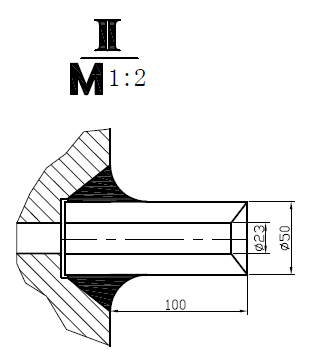
\includegraphics[width=1in]{切面2.png}
            %\caption{fig1}
        \end{minipage}
    }
    \subfigure[上封头切面]{
        \begin{minipage}[t]{0.25\linewidth}
            \centering
            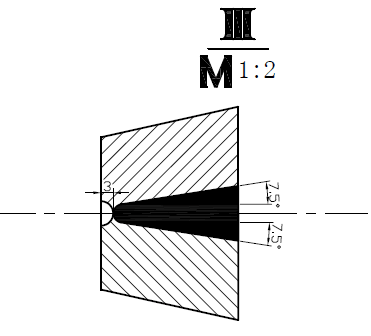
\includegraphics[width=1in]{切面3.png}
            %\caption{fig1}
        \end{minipage}
    }
    \subfigure[下封头切面]{
        \begin{minipage}[t]{0.25\linewidth}
            \centering
            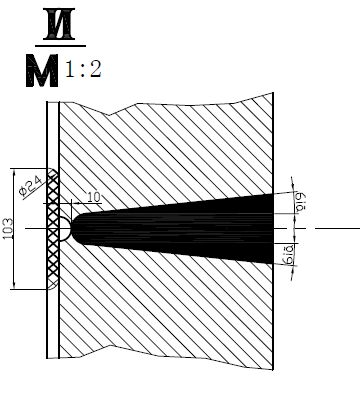
\includegraphics[width=1in]{切面4.jpg}
            %\caption{fig1}
        \end{minipage}
    }
    \subfigure[出水口切面]{
        \begin{minipage}[t]{0.25\linewidth}
            \centering
            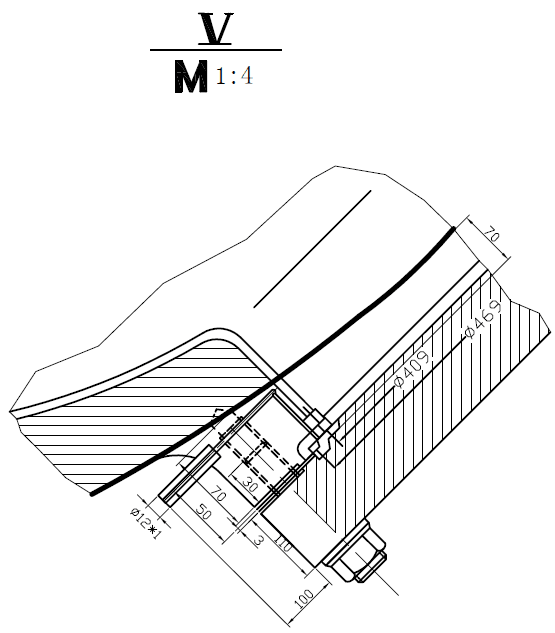
\includegraphics[width=1in]{切面5.png}
            %\caption{fig1}
        \end{minipage}
    }
\end{figure}

	\newpage
	\section{附件1 程序目录}
	\dirtree{%
    .1 /code.
    .2 CMakeLists.txt.
    .2 include.
    .3 CalculationOfAccelerationResistanceOfSecondaryCircuitWaterRisingSpace.h.
    .3 CalculationOfFrictionalResistanceInUTube.h.
    .3 CalculationOfLocalResistanceOfPrimaryCircuitWater.h.
    .3 CalculationOfResistanceOfFlowDistributionOrificeInSecondaryWaterRisingSpace.h.
    .3 CalculationOfResistanceOfSecondaryCircuitWaterVaporSeparator.h.
    .3 CalculationOfTheFrictionalResistanceOfTheSecondaryCircuitWaterRisingSpace.h.
    .3 CalculationOfTheLocalResistanceOfTheSecondaryCircuitWaterRisingSpace.h.
    .3 CalculationOfTheResistanceOfTheWaterBendInTheSecondaryCircuitWaterRiseSpace.h.
    .3 CalculationOfTheSpaceResistanceOfTheSecondaryCircuitWaterDrop.h.
    .3 CalculationOfTheTotalResistanceOfTheSecondaryCircuitWaterRisingSpace.h.
    .3 CalculationOfTotalResistanceOfPrimaryCircuitWater.h.
    .3 CalculationOfTotalResistanceOfSecondaryCircuitWaterCirculation.h.
    .3 GivenCondition.h.
    .3 HeatTransferCalculation.h.
    .3 HeatTransferTube.h.
    .3 LowerCylinder.h.
    .3 MainPipeInnerDiameter.h.
    .3 MotionHeadCalculation.h.
    .3 PreheatingSectionHeightCalculation.h.
    .3 SphericalBottomHead.h.
    .3 TubeBundleStructure.h.
    .3 UpperCylinder.h.
    .2 main.cpp.
    .2 src.
    .3 CalculationOfAccelerationResistanceOfSecondaryCircuitWaterRisingSpace.cpp.
    .3 CalculationOfFrictionalResistanceInUTube.cpp.
    .3 CalculationOfLocalResistanceOfPrimaryCircuitWater.cpp.
    .3 CalculationOfResistanceOfFlowDistributionOrificeInSecondaryWaterRisingSpace.cpp.
    .3 CalculationOfResistanceOfSecondaryCircuitWaterVaporSeparator.cpp.
    .3 CalculationOfTheFrictionalResistanceOfTheSecondaryCircuitWaterRisingSpace.cpp.
    .3 CalculationOfTheLocalResistanceOfTheSecondaryCircuitWaterRisingSpace.cpp.
    .3 CalculationOfTheResistanceOfTheWaterBendInTheSecondaryCircuitWaterRiseSpace.cpp.
    .3 CalculationOfTheSpaceResistanceOfTheSecondaryCircuitWaterDrop.cpp.
    .3 CalculationOfTheTotalResistanceOfTheSecondaryCircuitWaterRisingSpace.cpp.
    .3 CalculationOfTotalResistanceOfPrimaryCircuitWater.cpp.
    .3 CalculationOfTotalResistanceOfSecondaryCircuitWaterCirculation.cpp.
    .3 GivenCondition.cpp.
    .3 HeatTransferCalculation.cpp.
    .3 HeatTransferTube.cpp.
    .3 LowerCylinder.cpp.
    .3 MainPipeInnerDiameter.cpp.
    .3 MotionHeadCalculation.cpp.
    .3 PreheatingSectionHeightCalculation.cpp.
    .3 SphericalBottomHead.cpp.
    .3 TubeBundleStructure.cpp.
    .3 TubeSheet.cpp.
    .3 TubeSheet.h.
    .3 UpperCylinder.cpp.
}


\end{appendices}

\end{document}
